%% abtex2-modelo-trabalho-academico.tex, v-1.9.2 laurocesar
%% Copyright 2012-2014 by abnTeX2 group at http://abntex2.googlecode.com/ 
%%
%% This work may be distributed and/or modified under the
%% conditions of the LaTeX Project Public License, either version 1.3
%% of this license or (at your option) any later version.
%% The latest version of this license is in
%%   http://www.latex-project.org/lppl.txt
%% and version 1.3 or later is part of all distributions of LaTeX
%% version 2005/12/01 or later.
%%
%% This work has the LPPL maintenance status `maintained'.
%% 
%% The Current Maintainer of this work is the abnTeX2 team, led
%% by Lauro César Araujo. Further information are available on 
%% http://abntex2.googlecode.com/
%%
%% This work consists of the files abntex2-modelo-trabalho-academico.tex,
%% abntex2-modelo-include-comandos and abntex2-modelo-references.bib
%%

% ------------------------------------------------------------------------
% ------------------------------------------------------------------------
% abnTeX2: Modelo de Trabalho Academico (tese de doutorado, dissertacao de
% mestrado e trabalhos monograficos em geral) em conformidade com 
% ABNT NBR 14724:2011: Informacao e documentacao - Trabalhos academicos -
% Apresentacao
% ------------------------------------------------------------------------
% ------------------------------------------------------------------------

%-------------------------------------------------------------------------
% Modelo adaptado especificamente para o contexto do PPgSI-EACH-USP por 
% Marcelo Fantinato, com auxílio dos Professores Norton T. Roman, Helton
% H. Bíscaro e Sarajane M. Peres, em 2015, com muitos agradecimentos aos 
% criadores da classe e do modelo base.
%
% 20/06/2017: inclusão de "lista de quadros" com base no especificado em:
% https://github.com/abntex/abntex2/wiki/HowToCriarNovoAmbienteListing,
% de autoria de "Eduardo de Santana Medeiros Alexandre".
%
%-------------------------------------------------------------------------

\documentclass[
	% -- opções da classe memoir --
	12pt,				% tamanho da fonte
	% openright,			% capítulos começam em pág ímpar (insere página vazia caso preciso)
	oneside,			% para impressão apenas no anverso (apenas frente). Oposto a twoside
	a4paper,			% tamanho do papel. 
	% -- opções da classe abntex2 --
	%chapter=TITLE,		% títulos de capítulos convertidos em letras maiúsculas
	%section=TITLE,		% títulos de seções convertidos em letras maiúsculas
	%subsection=TITLE,	% títulos de subseções convertidos em letras maiúsculas
	%subsubsection=TITLE,% títulos de subsubseções convertidos em letras maiúsculas
	% -- opções do pacote babel --
	english,			% idioma adicional para hifenização
	%french,				% idioma adicional para hifenização
	%spanish,			% idioma adicional para hifenização
	brazil				% o último idioma é o principal do documento
	]{abntex2ppgsi}

% ---
% Pacotes básicos 
% ---
% \usepackage{lmodern}			% Usa a fonte Latin Modern			
% \usepackage[T1]{fontenc}		% Selecao de codigos de fonte.
\usepackage[utf8]{inputenc}		% Codificacao do documento (conversão automática dos acentos)
\usepackage{lastpage}			% Usado pela Ficha catalográfica
\usepackage{indentfirst}		% Indenta o primeiro parágrafo de cada seção.
\usepackage{color}				% Controle das cores
\usepackage{graphicx}			% Inclusão de gráficos
\usepackage{microtype} 			% para melhorias de justificação
\usepackage{pdfpages}     %para incluir pdf
\usepackage{algorithm}			%para ilustrações do tipo algoritmo
\usepackage{mdwlist}			%para itens com espaço padrão da abnt
\usepackage[noend]{algpseudocode}			%para ilustrações do tipo algoritmo


\usepackage{lscape}
\usepackage{longtable}
\usepackage{setspace}

\hyphenation{pro-ces-sa-men-to}

% ---
% Pacotes adicionais, usados apenas no âmbito do Modelo Canônico do abnteX2
% ---
\usepackage{lipsum}				% para geração de dummy text
% ---

% ---
% Pacotes de citações
% ---
\usepackage{hyperref}
\usepackage[brazilian,hyperpageref]{backref}	 % Paginas com as citações na bibl
\usepackage[alf,abnt-etal-list=0,abnt-etal-text=it]{abntex2cite}	% Citações padrão ABNT

% --- 
% CONFIGURAÇÕES DE PACOTES
% --- 

% ---
% Configurações do pacote backref
% Usado sem a opção hyperpageref de backref
\renewcommand{\backrefpagesname}{Citado na(s) página(s):~}
% Texto padrão antes do número das páginas
\renewcommand{\backref}{}
% Define os textos da citação
\renewcommand*{\backrefalt}[4]{
	\ifcase #1 %
		Nenhuma citação no texto.%
	\or
		Citado na página #2.%
	\else
		Citado #1 vezes nas páginas #2.%
	\fi}%
% ---

% ---
% Informações de dados para CAPA e FOLHA DE ROSTO
% ---

%-------------------------------------------------------------------------
% Comentário adicional do PPgSI - Informações sobre o ``instituicao'':
%
% Não mexer. Deixar exatamente como está.
%
%-------------------------------------------------------------------------
\instituicao{
	UNIVERSIDADE DE SÃO PAULO
	\par
	ESCOLA DE ARTES, CIÊNCIAS E HUMANIDADES
	\par
	PROGRAMA DE PÓS-GRADUAÇÃO EM SISTEMAS DE INFORMAÇÃO}

%-------------------------------------------------------------------------
% Comentário adicional do PPgSI - Informações sobre o ``título'':
%
% Em maiúscula apenas a primeira letra da sentença (do título), exceto 
% nomes próprios, geográficos, institucionais ou Programas ou Projetos ou 
% siglas, os quais podem ter letras em maiúscula também.
%
% O subtítulo do trabalho é opcional.
% Sem ponto final.
%
% Atenção: o título da Dissertação/Tese na versão corrigida não pode mudar. 
% Ele deve ser idêntico ao da versão original.
%
%-------------------------------------------------------------------------
\titulo{Classificação automática de espécies de abelhas por meio da morfologia de suas asas capturadas em imagens digitais utilizando rede neural convolucional}

%-------------------------------------------------------------------------
% Comentário adicional do PPgSI - Informações sobre o ``autor'':
%
% Todas as letras em maiúsculas.
% Nome completo.
% Sem ponto final.
%-------------------------------------------------------------------------
\autor{\uppercase{Danilo Souza de Assunção}}

%-------------------------------------------------------------------------
% Comentário adicional do PPgSI - Informações sobre o ``local'':
%
% Não incluir o ``estado''.
% Sem ponto final.
%-------------------------------------------------------------------------
\local{São Paulo}

%-------------------------------------------------------------------------
% Comentário adicional do PPgSI - Informações sobre a ``data'':
%
% Colocar o ano do depósito (ou seja, o ano da entrega) da respectiva 
% versão, seja ela a versão original (para a defesa) seja ela a versão 
% corrigida (depois da aprovação na defesa). 
%
% Atenção: Se a versão original for depositada no final do ano e a versão 
% corrigida for entregue no ano seguinte, o ano precisa ser atualizado no 
% caso da versão corrigida. 
% Cuidado, pois o ano da ``capa externa'' também precisa ser atualizado 
% nesse caso.
%
% Não incluir o dia, nem o mês.
% Sem ponto final.
%-------------------------------------------------------------------------
\data{2021}

%-------------------------------------------------------------------------
% Comentário adicional do PPgSI - Informações sobre o ``Orientador'':
%
% Se for uma professora, trocar por ``Profa. Dra.''
% Nome completo.
% Sem ponto final.
%-------------------------------------------------------------------------
\orientador{Prof. Dr. Helton Hideraldo Biscaro}

%-------------------------------------------------------------------------
% Comentário adicional do PPgSI - Informações sobre o ``Coorientador'':
%
% Opcional. Incluir apenas se houver co-orientador formal, de acordo com o 
% Regulamento do Programa.
%
% Se for uma professora, trocar por ``Profa. Dra.''
% Nome completo.
% Sem ponto final.
%-------------------------------------------------------------------------
\coorientador{Prof. Dr. Luciano Antonio Digiampietri}

\tipotrabalho{Dissertação (Mestrado)}

\preambulo{
%-------------------------------------------------------------------------
% Comentário adicional do PPgSI - Informações sobre o texto ``Versão 
% original'':
%
% Não usar para Qualificação.
% Não usar para versão corrigida de Dissertação/Tese.
%
%-------------------------------------------------------------------------
%Versão original \newline \newline \newline 
%-------------------------------------------------------------------------
% Comentário adicional do PPgSI - Informações sobre o ``texto principal do
% preambulo'':
%
% Para Doutorado, trocar por: Tese apresentada à Escola de Artes, Ciências e Humanidades da Universidade de São Paulo para obtenção do título de Doutor (ou Doutora) em Ciências pelo Programa de Pós-graduação em Sistemas de Informação. 
%
% Para Qualificação, trocar por: Projeto de pesquisa para exame de qualificação apresentado à Escola de Artes, Ciências e Humanidades da Universidade de São Paulo como parte dos requisitos para obtenção do título de Mestre (ou Doutor ou Doutora) em Ciências pelo Programa de Pós-graduação em Sistemas de Informação.
%
%-------------------------------------------------------------------------
%Dissertação apresentada à Escola de Artes, Ciências e Humanidades da Universidade de São Paulo para obtenção do título de Mestre em Ciências pelo Programa de Pós-graduação em Sistemas de Informação.
Texto de qualificação apresentado à Escola de Artes, Ciências e Humanidades da Universidade de São Paulo como etapa do mestrado no Programa de Pós-graduação em Sistemas de Informação.
%
\newline \newline Área de concentração: Metodologia e Técnicas da Computação
%-------------------------------------------------------------------------
% Comentário adicional do PPgSI - Informações sobre o texto da ``Versão 
% corrigida'':
%
% Não usar para Qualificação.
% Não usar para versão original de Dissertação/Tese.
% 
% Substituir ``xx de xxxxxxxxxxxxxxx de xxxx'' pela ``data da defesa''.
%
%-------------------------------------------------------------------------
\newline \newline \newline Versão corrigida contendo as alterações solicitadas pela comissão julgadora em xx de xxxxxxxxxxxxxxx de xxxx. A versão original encontra-se em acervo reservado na Biblioteca da EACH-USP e na Biblioteca Digital de Teses e Dissertações da USP (BDTD), de acordo com a Resolução CoPGr 6018, de 13 de outubro de 2011.}
% ---


% ---
% Configurações de aparência do PDF final

% alterando o aspecto da cor azul
\definecolor{blue}{RGB}{41,5,195}

% informações do PDF
\makeatletter
\hypersetup{
     	%pagebackref=true,
		pdftitle={\@title}, 
		pdfauthor={\@author},
    	pdfsubject={\imprimirpreambulo},
	    pdfcreator={laTeX com abnTeX2 adaptado para o PPgSI-EACH-USP},
		pdfkeywords={abnt}{latex}{abntex}{abntex2ppgsi}{qualificação de mestrado}{dissertação de mestrado}{qualificação de doutorado}{tese de doutorado}{ppgsi}, 
		colorlinks=true,       		% false: boxed links; true: colored links
    	linkcolor=blue,          	% color of internal links
    	citecolor=blue,        		% color of links to bibliography
    	filecolor=magenta,      		% color of file links
		urlcolor=blue,
		bookmarksdepth=4
}
\makeatother
% --- 

% --- 
% Espaçamentos entre linhas e parágrafos 
% --- 

% O tamanho do parágrafo é dado por:
\setlength{\parindent}{1.25cm}

% Controle do espaçamento entre um parágrafo e outro:
\setlength{\parskip}{0cm}  % tente também \onelineskip
\renewcommand{\baselinestretch}{1.5}

% ---
% compila o indice
% ---
\makeindex
% ---

	% Controlar linhas orfas e viuvas
  \clubpenalty10000
  \widowpenalty10000
  \displaywidowpenalty10000

% ----
% Início do documento
% ----
\begin{document}

% Retira espaço extra obsoleto entre as frases.
\frenchspacing 

% ----------------------------------------------------------
% ELEMENTOS PRÉ-TEXTUAIS
% ----------------------------------------------------------
% \pretextual

% ---
% Capa
% ---
%-------------------------------------------------------------------------
% Comentário adicional do PPgSI - Informações sobre a ``capa'':
%
% Esta é a ``capa'' principal/oficial do trabalho, a ser impressa apenas 
% para os casos de encadernação simples (ou seja, em ``espiral'' com 
% plástico na frente).
% 
% Não imprimir esta ``capa'' quando houver ``capa dura'' ou ``capa brochura'' 
% em que estas mesmas informações já estão presentes nela.
%
%-------------------------------------------------------------------------
\imprimircapa
% ---

% ---
% Folha de rosto
% (o * indica que haverá a ficha bibliográfica)
% ---
\imprimirfolhaderosto*
% ---

% ---
% Inserir a autorização para reprodução e ficha bibliografica
% ---

%-------------------------------------------------------------------------
% Comentário adicional do PPgSI - Informações sobre o texto da 
% ``autorização para reprodução e ficha bibliografica'':
%
% Página a ser usada apenas para Dissertação/Tese (tanto na versão original 
% quanto na versão corrigida).
%
% Solicitar a ficha catalográfica na Biblioteca da EACH. 
% Duas versões devem ser solicitadas, em dois momentos distintos: uma vez 
% para a versão original, e depois outra atualizada para a versão 
% corrigida.
%
% Atenção: esta página de ``autorização para reprodução e ficha 
% catalográfica'' deve ser impressa obrigatoriamente no verso da folha de 
% rosto.
%
% Não usar esta página para Qualificação.
%
% Substitua o arquivo ``fig_ficha_catalografica.pdf'' abaixo referenciado 
% pelo PDF elaborado pela Biblioteca
%
%-------------------------------------------------------------------------
% \begin{fichacatalografica}
%     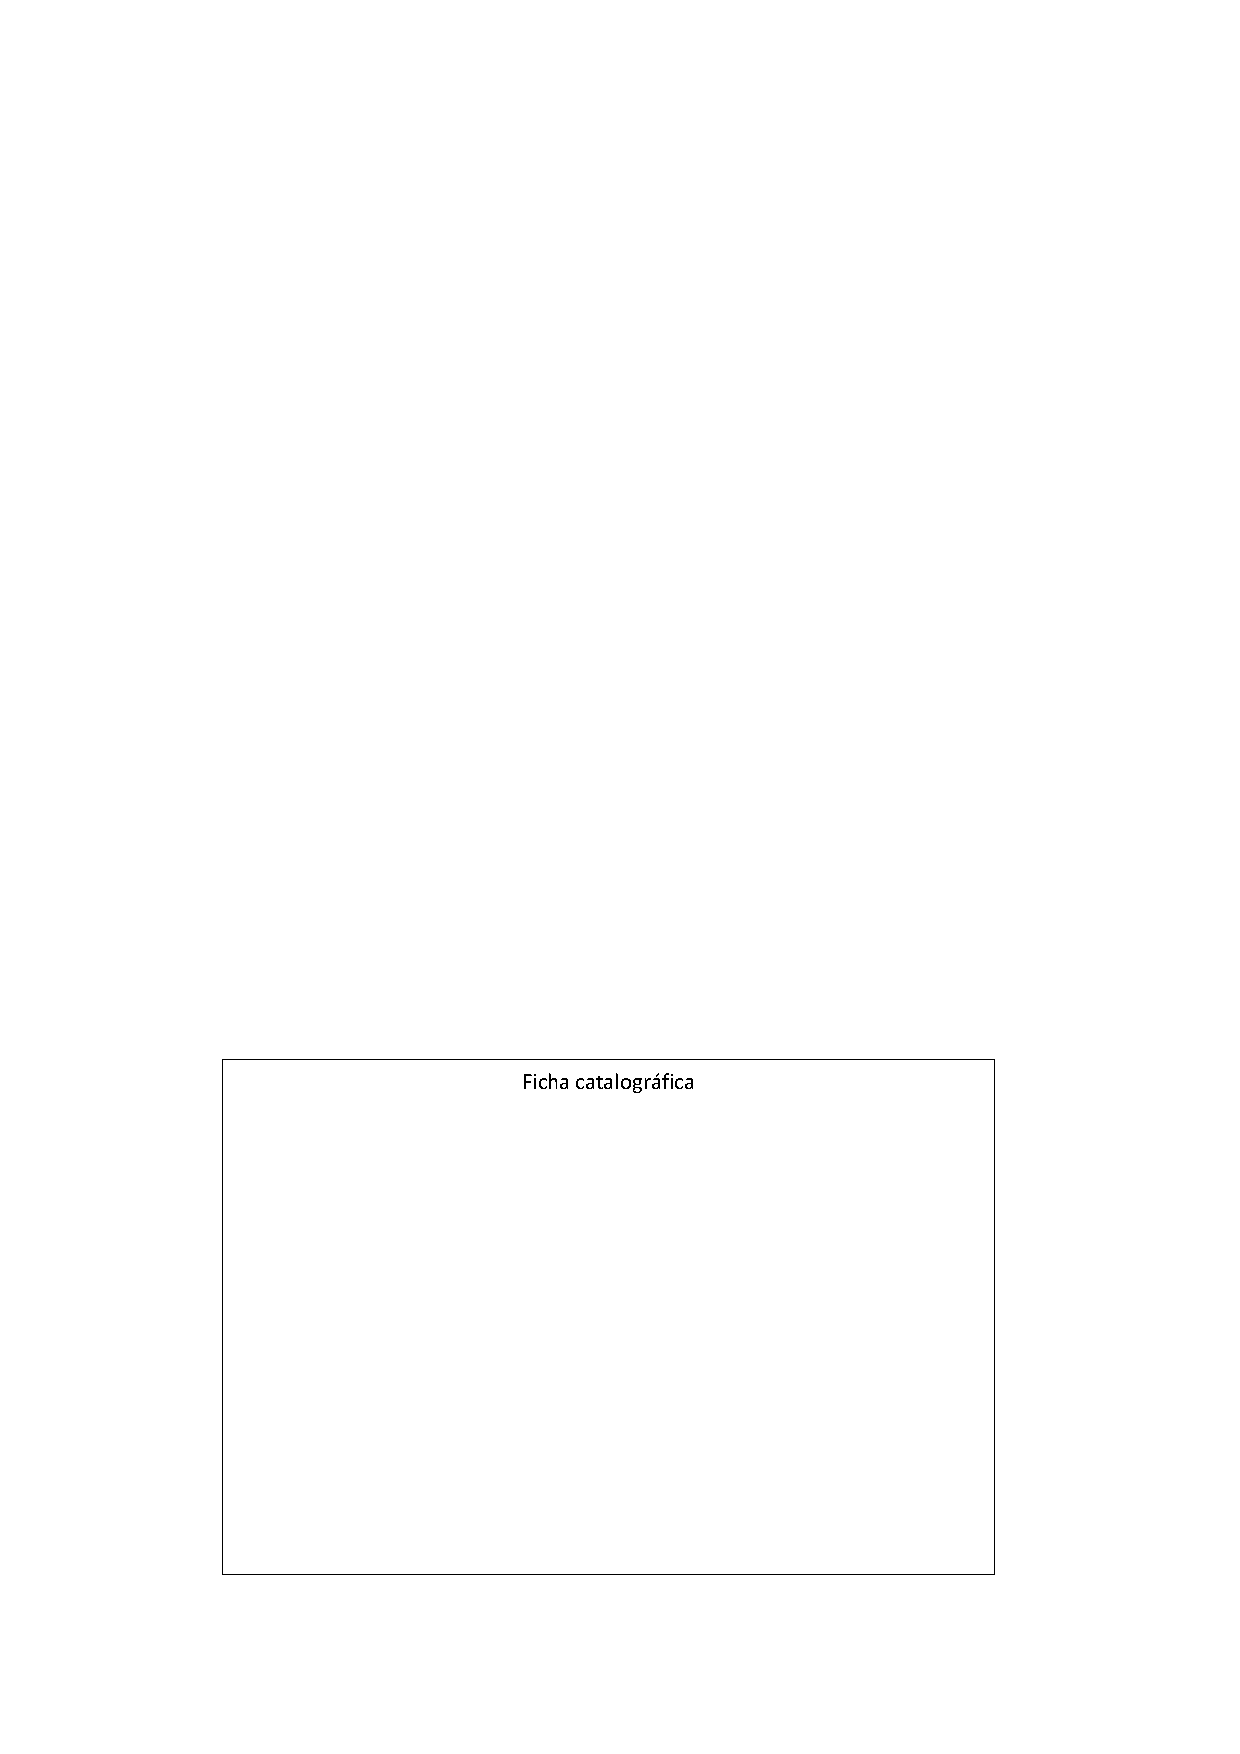
\includepdf{fig_ficha_catalografica.pdf}
% \end{fichacatalografica}

% ---
% Inserir errata
% ---
%-------------------------------------------------------------------------
% Comentário adicional do PPgSI - Informações sobre ``Errata'':
%
% Usar esta página de errata apenas em casos de excepcionais, e apenas 
% para a versão corrigida da Dissertação/Tese. Por exemplo, quando depois de
% já depositada e publicada a versão corrigida, ainda assim verifica-se
% a necessidade de alguma correção adicional.
%
% Se precisar usar esta página, busque a forma correta (o modelo correto) 
% para fazê-lo, de acordo com a norma ABNT.
%
% Não usar esta página para versão original de Dissertação/Tese.
% Não usar esta página para Qualificação.
%
%-------------------------------------------------------------------------
% \begin{errata}
% Elemento opcional para versão corrigida, depois de depositada.
% \end{errata}
% ---

% ---
% Inserir folha de aprovação
% ---

\begin{folhadeaprovacao}
%-------------------------------------------------------------------------
% Comentário adicional do PPgSI - Informações sobre ``Folha da aprovação'':
%
% Página a ser usada apenas para Dissertação/Tese.
%
% Não usar esta página para Qualificação.
%
% Substituir ``Fulano de Tal'' pelo nome completo do autor do trabalho, com 
% apenas as iniciais em maiúsculo.
%
% Substituir ``___ de ______________ de ______'' por: 
%     - Para versão original de Dissertação/Tese: deixar em branco, pois a data 
%       pode mudar, mesmo que ela já esteja prevista.
%     - Para versão corrigida de Dissertação/Tese: usar a data em que a defesa 
%       efetivamente ocorreu.
%
% Para Tese de Doutorado: trocar "Dissertação" por "Tese".
%-------------------------------------------------------------------------
\noindent Dissertação de autoria de Danilo Souza de Assunção, sob o título \textbf{``\imprimirtitulo''}, apresentada à Escola de Artes, Ciências e Humanidades da Universidade de São Paulo, para obtenção do título de Mestre em Ciências pelo Programa de Pós-graduação em Sistemas de Informação, na área de concentração Metodologia e Técnicas da Computação, aprovada em \rule{0.85cm}{0.5pt} de \rule{3.5cm}{0.5pt} de \rule{1.25cm}{0.5pt} pela comissão julgadora constituída pelos doutores:

\vspace*{3cm}

\begin{center}
%-------------------------------------------------------------------------
% Comentário adicional do PPgSI - Informações sobre ``assinaturas'':
%
% Para versão original de Dissertação/Tese: deixar em 
% branco (ou seja, assim como está abaixo), pois os membros da banca podem
% mudar, mesmo que eles já estejam previstos.
% 
% Para versão corrigida de Dissertação/Tese: usar os dados dos examinadores que 
% efetivamente participaram da defesa. 
% 
% Para versão corrigida de Dissertação/Tese: em caso de ``professora'', trocar 
% por ``Profa. Dra.'' 
% 
% Para versão corrigida de Dissertação/Tese: ao colocar os nomes dos 
% examinadores, usar seus nomes completos, exatamente conforme constam em 
% seus Currículos Lattes
% 
% Para a versão corrigida de Dissertação/Tese: remova o texto “Instituição: ”, 
% ou seja, coloque apenas/diretamente o nome da instituição, por exemplo 
% "Universidade de São Paulo" ou "Universidade Estadual de Campinas".
%
% Não abreviar os nomes das instituições.
%
% Verifique quantos membros há em sua banca, de acordo com o seu regulamento, 
% especificamente para o caso de Dissertação de Mestrado ou Tese de Doutorado, 
% e use o número correto de espaços para assinaturas.
%
%-------------------------------------------------------------------------

\assinatura{Prof. Dr. \\ Instituição \\ Presidente}

\assinatura{Prof. Dr. \\ Instituição}

\assinatura{Prof. Dr. \\ Instituição}

\assinatura{Prof. Dr. \\ Instituição}    % Incluir para bancas de tese de doutorado

\assinatura{Prof. Dr. \\ Instituição}    % Incluir para bancas de tese de doutorado

\end{center}
  
\end{folhadeaprovacao}
% ---

% ---
% Dedicatória
% ---
%-------------------------------------------------------------------------
% Comentário adicional do PPgSI - Informações sobre ``Dedicatória'': 
%
% Opcional para Dissertação/Tese.
% Não sugerido para Qualificação.
% 
%-------------------------------------------------------------------------
% \begin{dedicatoria}
%   \vspace*{\fill}
%   \centering
%   \noindent
%   \textit{Escreva aqui sua dedicatória, se desejar, ou remova esta página...} 
% 	 \vspace*{\fill}
% \end{dedicatoria}
% ---

% ---
% Agradecimentos
% ---
%-------------------------------------------------------------------------
% Comentário adicional do PPgSI - Informações sobre ``Agradecimentos'': 
%
% Opcional para Dissertação/Tese.
% Não sugerido para Qualificação.
% 
% 
% Financiamentos recebidos durante o projeto de mestrado/doutorado, vindos de qualquer 
% agência de fomento, devem ser mencionados na seção de agradecimentos da dissertação/tese. 
% Isso se aplica não apenas a bolsas de estudo, mas a qualquer tipo de financiamento, 
% tais como para apoio a participação em eventos, compra de materiais, traduções etc. 
% Especificamente para financiamento da Capes, siga as instruções contidas na portaria 
% 206, de 4/set/2018; para outras agências de fomento, procure as regras apropriadas.
%
% Portaria Capes 206, de 4/set/2018: 
% http://ppgsi.each.usp.br/arquivos/Portaria_0783227_Portaria_CAPES_DOU___206_de_2018.pdf 
%
%
%-------------------------------------------------------------------------
% \begin{agradecimentos}
% Texto de exemplo, texto de exemplo, texto de exemplo, texto de exemplo, texto de exemplo, texto de exemplo, texto de exemplo, texto de exemplo, texto de exemplo, texto de exemplo, texto de exemplo, texto de exemplo, texto de exemplo, texto de exemplo, texto de exemplo, texto de exemplo, texto de exemplo, texto de exemplo, texto de exemplo, texto de exemplo, texto de exemplo, texto de exemplo.

% Texto de exemplo, texto de exemplo, texto de exemplo, texto de exemplo, texto de exemplo, texto de exemplo, texto de exemplo, texto de exemplo, texto de exemplo, texto de exemplo, texto de exemplo, texto de exemplo, texto de exemplo, texto de exemplo, texto de exemplo, texto de exemplo, texto de exemplo, texto de exemplo, texto de exemplo, texto de exemplo, texto de exemplo, texto de exemplo.

% Texto de exemplo, texto de exemplo, texto de exemplo, texto de exemplo, texto de exemplo, texto de exemplo, texto de exemplo, texto de exemplo, texto de exemplo, texto de exemplo, texto de exemplo, texto de exemplo, texto de exemplo, texto de exemplo, texto de exemplo, texto de exemplo, texto de exemplo, texto de exemplo, texto de exemplo, texto de exemplo, texto de exemplo, texto de exemplo.

% Texto de exemplo, texto de exemplo, texto de exemplo, texto de exemplo, texto de exemplo, texto de exemplo, texto de exemplo, texto de exemplo, texto de exemplo, texto de exemplo, texto de exemplo, texto de exemplo, texto de exemplo, texto de exemplo, texto de exemplo, texto de exemplo, texto de exemplo, texto de exemplo, texto de exemplo, texto de exemplo, texto de exemplo, texto de exemplo.

% Texto de exemplo, texto de exemplo, texto de exemplo, texto de exemplo, texto de exemplo, texto de exemplo, texto de exemplo, texto de exemplo, texto de exemplo, texto de exemplo, texto de exemplo, texto de exemplo, texto de exemplo, texto de exemplo, texto de exemplo, texto de exemplo, texto de exemplo, texto de exemplo, texto de exemplo, texto de exemplo, texto de exemplo, texto de exemplo.
% \end{agradecimentos}
% ---

% ---
% Epígrafe
% ---
%-------------------------------------------------------------------------
% Comentário adicional do PPgSI - Informações sobre ``Epígrafe'': 
%
% Opcional para Dissertação/Tese.
% Não sugerido para Qualificação.
% 
%-------------------------------------------------------------------------
% \begin{epigrafe}
%     \vspace*{\fill}
% 	\begin{flushright}
% 		\textit{``Eu acredito muito na sorte. E tenho constatado que, quanto mais duro eu trabalho, mais sorte eu tenho.''\\
% 		(Thomas Jefferson)}
% 	\end{flushright}
% \end{epigrafe}
% ---

% ---
% RESUMOS
% ---

% resumo em português
\setlength{\absparsep}{18pt} % ajusta o espaçamento dos parágrafos do resumo
\begin{resumo}

%-------------------------------------------------------------------------
% Comentário adicional do PPgSI - Informações sobre ``referência'':
% 
% Troque os seguintes campos pelos dados de sua Dissertação/Tese (mantendo a 
% formatação e pontuação):
%   - SOBRENOME
%   - Nome1
%   - Nome2
%   - Nome3
%   - Título do trabalho: subtítulo do trabalho
%   - AnoDeDefesa
%
% Mantenha todas as demais informações exatamente como estão.
% 
% [Não usar essas informações de ``referência'' para Qualificação]
%
% Para Tese de Doutorado: trocar "Dissertação (Mestrado em Ciências)" por "Tese (Doutorado em Ciências)".
%-------------------------------------------------------------------------
\begin{flushleft}
ASSUNÇÃO, Danilo. \textbf{Classificação automática de espécies de abelhas por meio da morfologia de suas asas capturadas em imagens digitais utilizando rede neural convolucional}. \imprimirdata. \pageref{LastPage} f. Dissertação (Mestrado em Ciências) – Escola de Artes, Ciências e Humanidades, Universidade de São Paulo, São Paulo, 2022.
\end{flushleft}

O processo de classificação de espécies de abelhas é uma atividade importante para a preservação das abelhas, pois possibilita o estabelecimento de estratégias mais precisas de conservação ao obter informações detalhadas de uma determinada espécie e também para uma localidade específica. A realização automática da análise visual da morfologia das abelhas se convém devido às despesas necessárias nos processos de identificação manual, e, para esta análise morfológica, os conjuntos de características extraídos a partir das asas têm se mostrado uma eficiente maneira para a identificação das espécies utilizando métodos estatísticos ou computacionais. O aprendizado profundo tem sido amplamente aplicado em atividades relacionadas à visão computacional. Diferente dos métodos tradicionais de aprendizado de máquina, o modelo de aprendizado profundo pode aprender recursos automaticamente a partir de uma grande quantidade de amostras de dados, e não requer a assistência de um especialista no domínio para a extração destas características. No aprendizado profundo, as Redes Neurais Convolucionais (CNN) são bem conhecidas por seu sucesso em muitas tarefas de visão computacional. Neste trabalho será desenvolvido um método utilizando CNN para classificação de espécies de abelhas através da morfologia de suas asas presente em imagens digitais.

Palavras-chaves: Redes Neurais Convolucionais. CNN. Aumento de dados. Aprendizado por transferência. Reconhecimento de espécies. Reconhecimento de espécies de abelhas. Morfologia das asas. Reconhecimento por imagens digitais.
\end{resumo}

% resumo em inglês
%-------------------------------------------------------------------------
% Comentário adicional do PPgSI - Informações sobre ``resumo em inglês''
% 
% Caso a Qualificação ou a Dissertação/Tese inteira seja elaborada no idioma inglês, 
% então o ``Abstract'' vem antes do ``Resumo''.
% 
%-------------------------------------------------------------------------
\begin{resumo}[Abstract]
\begin{otherlanguage*}{english}

%-------------------------------------------------------------------------
% Comentário adicional do PPgSI - Informações sobre ``referência em inglês''
% 
% Troque os seguintes campos pelos dados de sua Dissertação/Tese (mantendo a 
% formatação e pontuação):
%     - SURNAME
%     - FirstName1
%     - MiddleName1
%     - MiddleName2
%     - Work title: work subtitle
%     - DefenseYear (Ano de Defesa)
%
% Mantenha todas as demais informações exatamente como estão.
%
% [Não usar essas informações de ``referência'' para Qualificação]
%
%-------------------------------------------------------------------------
\begin{flushleft}
ASSUNÇÃO, Danilo. \textbf{Classificação automática de espécies de abelhas por meio da morfologia de suas asas capturadas em imagens digitais utilizando rede neural convolucional}. \imprimirdata. \pageref{LastPage} p. Dissertation (Master of Science) – School of Arts, Sciences and Humanities, University of São Paulo, São Paulo, 2022.
\end{flushleft}

Bees' species classification process turns out to be an important activity in bee preservation, as it makes it possible to establish more precise conservation strategies when obtaining detailed information about a specific species and also for a specific location. The automatic realization of the visual analysis of the morphology of the bees is convenient due to the necessary expenses in the processes of manual identification, and, for this morphological analysis, the sets of characteristics extracted from the wings have shown to be an efficient way for the identification of the species using statistical methods. Deep learning has been widely applied in activities related to computer vision. Unlike traditional machine learning methods, the deep learning model can automatically learn resources from a large number of data samples and does not require the assistance of an expert in the field to extract these characteristics. In deep learning, Convolutional Neural Networks (CNN) are well known for their success in many computer vision tasks. In this work, a method will be developed using CNN to classify bee species through the morphology of their wings present in digital images.

Keywords: Convolutional Neural Networks. CNN. Data augmentation. Transfer learning. Species recognition. Recognition of bee species. Wing morphology. Digital image recognition.
\end{otherlanguage*}
\end{resumo}

% ---
% ---
% inserir lista de figuras
% ---
\pdfbookmark[0]{\listfigurename}{lof}
\listoffigures*
\cleardoublepage
% ---

% ---
% inserir lista de algoritmos
% ---
% \pdfbookmark[0]{\listalgorithmname}{loa}
% \listofalgorithms
% \cleardoublepage

% ---
% inserir lista de quadros
% ---
% \pdfbookmark[0]{\listofquadrosname}{loq}
% \listofquadros*
% \cleardoublepage


% ---
% inserir lista de tabelas
% ---
\pdfbookmark[0]{\listtablename}{lot}
\listoftables*
\cleardoublepage
% ---

% ---
% inserir lista de abreviaturas e siglas
% ---
%-------------------------------------------------------------------------
% Comentário adicional do PPgSI - Informações sobre ``Lista de abreviaturas 
% e siglas'': 
%
% Opcional.
% Uma vez que se deseja usar, é necessário manter padrão e consistência no
% trabalho inteiro.
% Se usar: inserir em ordem alfabética.
%
%-------------------------------------------------------------------------
\begin{siglas}
  \item[ANN] Artificial Neural Network
  \item[CNN] Convolutional Neural Network
  \item[GAN] Generative Adversarial Networks
  \item[MNIST] Modified National Institute of Standards and Technology
  \item[RBF] Radius Basis Function
  \item[ReLU] Rectified Linear Unit
  \item[RGB] Red, Green and Blue
  \item[ResNet] Residual Neural Network
  \item[SVM] Support Vector Machine
  \item[VGG] Visual Geometry Group
\end{siglas}
% ---

% ---
% inserir lista de símbolos
% ---
%-------------------------------------------------------------------------
% Comentário adicional do PPgSI - Informações sobre ``Lista de símbolos'': 
%
% Opcional.
% Uma vez que se deseja usar, é necessário manter padrão e consistência no
% trabalho inteiro.
% Se usar: inserir na ordem em que aparece no texto.
% 
%-------------------------------------------------------------------------
\begin{simbolos}
  \item[$ A\textsubscript{c} $] Acurácia
  \item[$ F\textsubscript{1} $] Medida F
  \item[$ F\textsubscript{n} $] Falso negativo
  \item[$ F\textsubscript{r} $] Falso positivo
  \item[$ P\textsubscript{r} $] Precisão
  \item[$ R\textsubscript{v} $] Revocação
  \item[$ V\textsubscript{n} $] Verdadeiro negativo
  \item[$ V\textsubscript{p} $] Verdadeiro positivo
\end{simbolos}
% ---

% ---
% inserir o sumario
% ---
\pdfbookmark[0]{\contentsname}{toc}
\tableofcontents*
\cleardoublepage
% ---



% ----------------------------------------------------------
% ELEMENTOS TEXTUAIS
% ----------------------------------------------------------
\textual



%-------------------------------------------------------------------------
% Comentário adicional do PPgSI - Informações sobre ``títulos de seções''
% 
% Para todos os títulos (seções, subseções, tabelas, ilustrações, etc.):
%
% Em maiúscula apenas a primeira letra da sentença (do título), exceto 
% nomes próprios, geográficos, institucionais ou Programas ou Projetos ou
% siglas, os quais podem ter letras em maiúscula também.
%
%------------------------------------------------------------------------

% ----------------------------------------------------------
% CAPITULO - INTRODUÇÃO
% ----------------------------------------------------------
\chapter{Introdução}
As plantações alimentícias possuem uma elevada dependência  em relação as abelhas, cuja a responsabilidade de polinização se encontra por volta de 70\% \cite{drauschke2007reliable}, ou seja, as abelhas economizam um serviço no qual custariam cerca de 65 bilhões de dólares anualmente \cite{pimentel1997economic}. Sendo elas também responsáveis por um papel de extrema valia para a natureza, onde a preservação de ecossistemas terrestres em conjunto de seu relacionamento com as abelhas \cite{lawton1998daily}. 

Diante disso, o processo de classificação de espécies de abelhas acaba por ser um importante sistema para a sua preservação, por obter informações detalhadas e possibilitando estabelecer estratégias mais precisas de conservação de uma determinada espécie e também para uma localidade especifica \cite{goulson2015bee}. 

A realização automática da análise visual da morfologia das abelhas se convêm devido as despesas necessárias nos processos de identificação manual, e para esta análise morfológica, os conjuntos de características extraídos a partir das asas têm se mostrado uma maneira eficiente para a identificação das espécies utilizando métodos estatísticos \cite{francoy2008identification}.

O aprendizado profundo tem sido amplamente utilizado em atividades relacionadas à visão computacional. É um ramo do aprendizado de máquina, baseado na aplicação de uma grande quantidade de dados para treinamento de um modelo. Diferente dos métodos tradicionais de aprendizado de máquina, o modelo de aprendizado profundo pode aprender recursos automaticamente a partir de uma grande quantidade de amostras de dados, e não requer a assistência de um especialista no domínio para extração destas características \cite{liu2020classification}. No aprendizado profundo, as redes neurais convolucionais (CNN) são bem conhecidas por seu sucesso em muitas tarefas de visão computacional. \cite{le2020automated}.

Devido a inevitável presença de uma grande quantidade de dados para o treinamento deste tipo de rede, é essencial que, para conjuntos de dados menores, se tenha o auxilio de técnicas que permitam atingir bons resultados. Baseado nisso, serão adicionados a este trabalho, mecanismos de aumento de dados ou aprendizado por transferência, afim de se obter uma melhor convergência do modelo por meio da CNN com relação ao conjunto de dados das asas de abelhas disponibilizados para identificação de suas respectivas espécies.

\section{Hipótese}
O uso de CNN para automatização do processo de extração de características e classificação, podem trazer resultados promissores ao problema em questão, devido a sua capacidade de identificar e extrair características com mais qualidade das imagens.

Esta hipótese será testada levando em consideração as medidas obtidas a partir de métricas tradicionais de aprendizado de máquina do modelo proposto, e relacionando com o modelos de \textit{baseline} adquiridos como o apresentado por \citeonline{liu2020classification}. 

Espera-se que o modelo proposto apresente resultados superiores aos modelos de \textit{baseline} para as métricas sugeridas.

\section{Objetivos}
Este projeto de pesquisa tem como objetivo o desenvolvimento de uma ferramenta de classificação de espécies de abelhas por meio da morfologia de suas asas, utilizando uma CNN como mecanismo de extração de características e classificação destas imagens, junto à utilização de técnicas de aumento de dados ou aprendizado por transferência para otimização dos resultados da rede, afim de se obter melhores resultados que os modelos de \textit{baseline} definidos. Desta forma, este trabalho tem como objetivos específicos as seguintes entregas:

\begin{enumerate}
  \item Conjunto de técnicas para aplicação de aumento de dados do conjunto atual disponibilizado;
  \item Extrator automático de características das imagens das asas das abelhas;
  \item Mecanismo de classificação e validação das espécies de abelhas.
\end{enumerate}

\section{Justificativa}
Uma vez que o conjunto demonstre cenários de sucesso com base nas avaliações aplicadas, tornará-se evidente que a aplicação de uma CNN poderá atingir um modelo mais próximo do estado da arte para o problema abordado.

\section{Estrutura do documento}
O restante deste documento está organizado da seguinte forma. O capítulo 2 descreve os conceitos fundamentais para o entendimento do trabalho. O capítulo 3 apresenta a revisão de literatura realizada. O capítulo 4 descreve o conjunto de dados e as técnicas a serem utilizadas. O capítulo 5 aborda a proposta de pesquisa. Por fim, o capítulo 6 contém as considerações finais acerca do projeto.

% ----------------------------------------------------------
% CAPITULO - CONCEITOS FUNDAMENTAIS
% ----------------------------------------------------------
\chapter{Conceitos fundamentais}
Neste capítulo são apontados alguns tópicos elementares para a compreensão deste projeto. Dessa forma, primeiro é realizada uma curta introdução ao tema de visão computacional, logo depois são apresentados as definições referentes à aprendizado de máquina, aprendizado profundo, redes neurais artificiais, redes neurais convolucionais (CNN), técnicas de aprendizado por transferência e aumento de dados.

\section{Visão computacional}
A visão computacional é a ciência responsável pela visão de uma máquina, diante da forma como um computador visualiza o ambiente à sua volta, extraindo informações significativas a partir de imagens capturadas por dispositivos eletrônicos como câmeras digitais. 

Neste contexto, uma imagem pode ser definida como um conjunto de pontos, chamados \textit{pixels}, que são a menor parte da imagem. Cada \textit{pixel} possui uma cor e uma coordenada na imagem. A resolução da imagem corresponde a quantidade de pixel sem cada uma de suas dimensões. Ou seja, uma imagem com resolução de 1024 por 768, comumente representada como “1024 x 768”, tem 1024 \textit{pixels} no eixo horizontal e 768 na vertical.

Com o uso da visão computacional, é possível reconhecer, manipular e refletir sobre os componentes que compõem uma imagem. Dessa forma, a visão computacional fornece ao computador uma infinidade de informações precisas a partir de imagens e vídeos, de forma que o computador consiga executar determinadas tarefas ao simular o comportamento visual do ser humano. Para um modelo de visão computacional, tem-se a composição de determinadas etapas, sendo elas, aquisição de imagem, pré-processamento, segmentação, extração de características e classificação:

\begin{itemize}
  \item Aquisição de imagem: trata-se do processo de obtenção de uma ou várias imagens a partir de dispositivos eletrônicos como câmeras digitais ou escâneres, onde os \textit{pixels} em cada imagem obtida ( bidimensional, tridimensional ou uma sequência de imagens) indica suas características de propriedades físicas capturadas.
  \item Pré-processamento: é um processo realizado para ajuste ou normalização de imagens, além de preparar tais imagens para a utilização em algoritmos de aprendizado de máquina, tendo como exemplo, destaques de contornos, bordas, destaques de figuras geométricas, remoção de ruídos, normalização de tom da imagem, redução dos canais de cores para o tom de cinza, alteração do brilho e contraste e dentre outras técnicas.
  \item Segmentação: é um mecanismo que permite dividir em segmentos uma imagem, destacando objetos e alterando a representação da imagem, para que o processo de reconhecimento de padrões seja realizado com mais acurácia ou até mesmo para que este processo de reconhecimento de padrões seja possível.
  \item Extração de características: é um processo que constitui a extração das composições de uma imagem, obtendo matematicamente tais características como textura, bordas ou formatos.
  \item Classificação: é o método que inclui a validação da satisfação dos dados obtidos, a estimativa de parâmetros sobre a imagem e a classificação dos objetos obtidos em diferentes categorias.
\end{itemize}

\section{Aprendizado de máquina}
Dentre as definições presentes na literatura, \citeonline{mohri2018foundations} diz que, o aprendizado de máquina pode ser amplamente definido como métodos computacionais, usando a experiência para melhorar o desempenho ou realizar previsões precisas. A experiência se refere às informações anteriores disponíveis para o modelo de aprendizagem de máquina, que normalmente assumem a forma de dados eletrônicos coletados e disponibilizados para análise. Esses dados podem estar na forma de conjuntos de treinamento com identificação humana ou a diferentes tipos de informações obtidas por meio da interação com o ambiente. Em todos os casos, sua qualidade e tamanho são cruciais para o sucesso das previsões feitas pelo modelo.

O aprendizado de máquina consiste em projetar algoritmos de previsão eficientes e precisos \cite{mohri2018foundations}. Como em outras áreas da ciência da computação, algumas medidas críticas sobre a qualidade desses algoritmos são a sua complexidade de tempo e espaço \cite{mohri2018foundations}.

Como o sucesso de um algoritmo de aprendizado depende dos dados usados, o aprendizado de máquina está inerentemente relacionado à análise de dados e estatísticas \cite{mohri2018foundations}. De maneira mais geral, as técnicas de aprendizagem são métodos orientados por dados que combinam conceitos fundamentais em ciência da computação com ideias de estatística, probabilidade e otimização \cite{mohri2018foundations}.

\subsection{Tarefas padrões em aprendizado de máquina}
A seguir estão algumas tarefas comumente aplicadas no campo de aprendizado de máquina:

\begin{itemize}
  \item Classificação (\textit{Classification}): trata-se do problema de atribuir uma categoria a cada item \cite{mohri2018foundations}. Por exemplo, a classificação de imagens consiste em atribuir a cada imagem uma categoria como carro, navio ou avião. O número de categorias em tais tarefas costuma ser menor do que algumas centenas, mas pode ser muito maior em algumas tarefas difíceis, e até mesmo ilimitado, como em classificação de texto ou reconhecimento de fala \cite{mohri2018foundations}.

  \item Regressão (\textit{Regression}): é a atividade de solucionar problemas já previstos a partir de dados históricos de cada item \cite{mohri2018foundations}. Exemplos de regressão incluem a previsão de valores de estoque ou variações de variáveis econômicas. Na regressão, a penalidade para uma previsão incorreta depende da magnitude da diferença entre os valores verdadeiros e previstos, visto que, em contraste com o problema de classificação, onde normalmente não há noção de proximidade entre as várias categorias \cite{mohri2018foundations}.

  \item Ranqueamento (\textit{Ranking}): proporciona à resolução do problema de aprender a ordenar os itens de acordo com algum critério \cite{mohri2018foundations}. A pesquisa na web, por exemplo, ao retornar páginas da web relevantes para uma consulta de pesquisa, é o exemplo de classificação canônica. Muitos outros problemas de classificação semelhantes, surgem no contexto do projeto de extração de informações ou sistemas de processamento de linguagem natural \cite{mohri2018foundations}.

  \item Clusterização (\textit{Clustering}): é uma forma de solucionar o problema de particionar um conjunto de itens em subconjuntos homogêneos \cite{mohri2018foundations}. A clusterização é frequentemente utilizada para analisar conjuntos de dados muito grandes \cite{mohri2018foundations}. Por exemplo, no contexto da análise de rede social, os algoritmos de agrupamento tentam identificar comunidades naturais dentro de grandes grupos de pessoas \cite{mohri2018foundations}.

  \item Redução da dimensionalidade (\textit{Dimensionality reduction}): consiste em transformar uma representação inicial de itens em uma representação de dimensão inferior, preservando algumas propriedades da representação inicial \cite{mohri2018foundations}. Um exemplo comum envolve o pré-processamento de imagens digitais em tarefas de visão computacional.
\end{itemize}

\subsection{Terminologias}
A seguir está uma lista de definições e terminologias comumente usados no escopo de aprendizado de máquina:

\begin{itemize}
  \item Amostras (\textit{Examples}): itens ou instâncias de dados usados para aprendizagem ou avaliação em um modelo de aprendizado de máquina \cite{mohri2018foundations}.
  
  \item Características (\textit{Features}): O conjunto de atributos, frequentemente representado como um vetor, associado a uma amostra \cite{mohri2018foundations}. No caso de uma imagem, alguns recursos relevantes podem incluir a forma do objeto presente nesta imagem, cor e dentre vários outros aspectos.
  
  \item Rótulo ou Classe (\textit{Label}): valores ou categorias atribuídos a exemplos \cite{mohri2018foundations}. Em problemas de classificação, as amostras são atribuídas a categorias específicas. Por exemplo, dado imagens de objetos de veículos, se tem categorias de carro, avião ou navio, num cenário onde é tido um problema de classificação com múltiplas classes.
  
  \item Hiperparâmetros (\textit{Hyperparameters}): parâmetros livres que não são determinados pelo algoritmo de aprendizagem, mas sim especificados como entrada para o algoritmo de aprendizagem \cite{mohri2018foundations}.

  \item Amostra de treinamento (\textit{Training sample}): são amostras utilizadas para treinar um algoritmo de aprendizagem \cite{mohri2018foundations}. Em um problema envolvendo reconhecimento de padrões por meio de imagens digitais, a amostra de treinamento consiste em um conjunto de exemplos de imagens junto a suas classes associadas.

  \item Amostra de validação (\textit{Validation sample}): são exemplos usados para ajustar os parâmetros de um algoritmo de aprendizagem ao trabalhar com dados rotulados \cite{mohri2018foundations}. A amostra de validação é usada para selecionar valores apropriados para os parâmetros livres do algoritmo de aprendizagem (hiperparâmetros) \cite{mohri2018foundations}.

  \item Amostra de teste (\textit{Test sample}): são exemplos usados para avaliar o desempenho de um algoritmo de aprendizagem \cite{mohri2018foundations}. A amostra de teste é separada dos dados de treinamento e validação, não sendo disponibilizada na fase de aprendizado \cite{mohri2018foundations}. Por exemplo, em um cenário de reconhecimento facial, a amostra de teste consiste em uma coleção de exemplos de imagens de rostos, para os quais o algoritmo de aprendizagem deve prever suas determinadas classes com base em recursos, sendo então comparadas com os rótulos da amostra de teste para medir o desempenho do algoritmo.

  \item Função de perda (\textit{Loss function}): é um tipo de função que mede a diferença, ou perda, entre uma classe prevista e uma classe verdadeira de uma determinada amostra \cite{mohri2018foundations}.
\end{itemize}

\subsection{Cenários de aprendizagem}
Nesta subseção, será descrito alguns cenários de aprendizado de máquina que podem ser interpretados como tipos de treinamento. Esses cenários diferem nos tipos de dados de treinamento disponíveis para o modelo de aprendizagem, na ordem e no método pelo qual os dados de treinamento são recebidos, e nos dados de teste usados para avaliar o algoritmo de aprendizagem.

\begin{itemize}
  \item Aprendizagem supervisionada (\textit{Supervised learning}): aprendizagem supervisionada é a aprendizagem por meio de entradas pré-rotuladas, atuando como alvos, e, tem como objetivo, a utilização de treinamentos para a redução de erros de classificação dos modelos, fazendo uso do cálculo correto do valor de saída do treinamento \cite{o2015introduction}. Haverá um conjunto de valores de entrada (vetores) para cada modelo de treinamento, e um ou mais valores de saída associados \cite{o2015introduction}. O objetivo desta forma de treinamento é reduzir o erro geral de classificação dos modelos, por meio do cálculo correto do valor de saída do treinamento \cite{o2015introduction}.
  
  \item Aprendizagem não supervisionada (\textit{Unsupervised learning}): a aprendizagem não supervisionada diverge do modelo supervisionado devido ao conjunto de treinamento não incluir nenhuma classe \cite{o2015introduction}. A capacidade da rede em reduzir ou aumentar uma função de custo associada são as determinantes para o sucesso \cite{o2015introduction}. No entanto, nota-se que a grande parte das tarefas de reconhecimentos de padrões com foco em imagens, geralmente dependem de classificação usando aprendizado supervisionado \cite{o2015introduction}.
\end{itemize}

\subsection{Sobreajuste e subajuste}
O objetivo de um modelo de aprendizado de máquina é aproximar uma função desconhecida que associe elementos de entrada aos de saída (para um classificador, os chamamos de classes) \cite{bonaccorso2017machine}. No entanto, um conjunto de treinamento é normalmente uma representação de uma distribuição global, sendo que, esta distribuição não pode conter todos os elementos possíveis, caso contrário, o problema poderia ser resolvido com uma associação de um para um \cite{bonaccorso2017machine}. Portanto, ao treinar o modelo, é necessário pensar em ajustá-lo, mas mantendo-o livre para generalizar quando uma entrada desconhecida é apresentada. Infelizmente, essa condição ideal nem sempre é fácil de se alcançar, e este comportamento ocorre devido à duas características eminentes que são:

\begin{itemize}
  \item Sobreajuste (\textit{Overfitting}): o modelo não é mais capaz de generalizar, considerando a dinâmica original fornecida pelo conjunto de treinamento \cite{bonaccorso2017machine}. Ele pode associar quase perfeitamente todas as amostras conhecidas aos valores de saída correspondentes, mas quando uma entrada desconhecida é apresentada, o erro de predição correspondente pode ser muito alto \cite{bonaccorso2017machine}.

  \item Subajuste (\textit{Underfitting}): isso significa que o modelo não é capaz de capturar a dinâmica mostrada pelo mesmo conjunto de treinamento (provavelmente porque sua capacidade é muito limitada) \cite{bonaccorso2017machine}.
\end{itemize}

Na Figura \ref{fig:subajuste_sobreajuste} é possível observar os efeitos negativos causados pelo subajuste e sobreajuste. No gráfico da esquerda o efeito de subajuste mostra a incapacidade do modelo em capturar a dinâmica presente no modelo de treinamento, obtendo resultados ruins já neste procedimento. No gráfico localizado ao meio, temos um cenário adequado onde o modelo foi capaz de generalizar totalmente a distribuição apresentada. Por fim, no gráfico à direita, temos um cenário de sobreajuste, onde é possível verificar que, em determinados momentos ele é capaz de se adaptar, indicando assim os valores do conjunto de treinamento fornecido, mas para outros cenários do quadro de distribuição, ele não possui a mesma capacidade de identificação.

\begin{figure}[H]
    \centering
    \caption{Representação gráfica de subajuste e sobreajuste}
    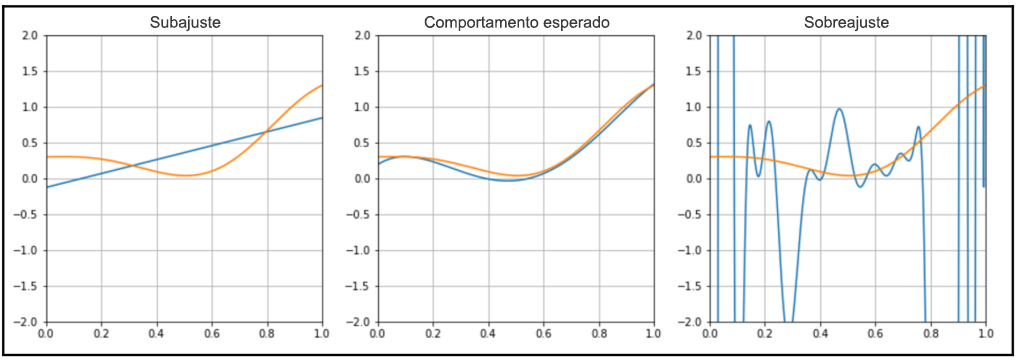
\includegraphics[scale=.45]{imagens/conceitos_basicos/subajuste_sobreajuste.jpg}
    \label{fig:subajuste_sobreajuste}
    \source{\citeonline{bonaccorso2017machine}}
\end{figure}

\subsection{Avaliação de desempenho de classificadores}
Ao categorizar uma amostra baseada em um algoritmo de classificação, pode-se determinar que tal amostra pertence a um dos quatro itens seguintes:

\begin{itemize}
  \item Verdadeiro positivo (V\textsubscript{p})
  \item Verdadeiro negativo (V\textsubscript{n})
  \item Falso positivo (F\textsubscript{p})
  \item Falso negativo (F\textsubscript{n})
\end{itemize}

Tendo como exemplo, um Verdadeiro positivo entraria para uma classe determinada pelo classificador, identificando-a como pertencente à classe C. Em sequência, Verdadeiro negativo será o resultado do processo inverso, onde classificador identificaria a amostra como sendo não pertencente à classe C. O falso positivo se dá quando ocorre um erro pelo classificador, onde a identificação de uma amostra é determinada como sendo da classe C, sendo que ela não é . Em suma, o falso negativo são amostras nas quais o classificador não pode identificar, ou então as classificou como pertencente à outra classe.

Para fins de medição de qualidade do modelo de aprendizado de máquina, é utilizado funções de avaliação de classificadores. As funções mais usuais entre elas são:

\begin{itemize}
  \item Precisão (P\textsubscript{r})
  \item Revocação (R\textsubscript{v})
  \item Medida F (F\textsubscript{1})
  \item Acurácia (A\textsubscript{c})
\end{itemize}

Precisão (P\textsubscript{r}) é a parcela de amostras nas quais obtiveram uma identificação e classificação corretamente. Podendo ser descrita a partir de seu cálculo pela Fórmula \ref{equation_precisao}.

\begin{equation}
  P\textsubscript{r}=\frac{V\textsubscript{p}}{V\textsubscript{p}+F\textsubscript{p}}
  \label{equation_precisao}
\end{equation}

Revocação (R\textsubscript{v}) é a parcela de amostras com identificação correta, onde pertencem a uma determinada classe entre todas as amostra desta mesma classe. Seu cálculo pode ser descrito a partir da Fórmula \ref{equation_revocacao}.

\begin{equation}
  R\textsubscript{v}=\frac{V\textsubscript{p}}{V\textsubscript{p}+F\textsubscript{n}}
  \label{equation_revocacao}
\end{equation}

Medida F (F\textsubscript{1}) é a busca da média harmônica entre a precisão e a revocação. O valor da medição torna-se ideal quanto mais próximo de 0,5, enquanto que, quanto mais próximo de 0, expressa um resultado ruim. Sua equação pode ser descrita pela Fórmula \ref{equation_medida_f}.

\begin{equation}
  F\textsubscript{1}=2\frac{P\textsubscript{r}R\textsubscript{v}}{P\textsubscript{r}+R\textsubscript{v}}
  \label{equation_medida_f}
\end{equation}

Acurácia (A\textsubscript{c}) é a classificação correta sobre as parcelas de amostras, se elas pertencem ou não a uma classe, diante de todas as amostras testadas. Denominando assim a porcentagem de classificação correta das amostras. Sua equação pode ser descrita pela Fórmula \ref{equation_acuracia}.

\begin{equation}
  A\textsubscript{c}=\frac{V\textsubscript{p}+V\textsubscript{n}}{V\textsubscript{p}+V\textsubscript{n}+F\textsubscript{p}+F\textsubscript{n}}
  \label{equation_acuracia}
\end{equation}

\section{Aprendizado profundo}
Dentre as diversas definições presentes, no artigo de \citeonline{lecun2015deep}, o aprendizado profundo é dito como um conjunto de algoritmos que modelam abstrações de alto nível de dados usando uma hierarquia com várias camadas de processamento, sendo esta uma forma de aprendizado de máquina. Como o computador reúne conhecimento com base na experiência, não há necessidade de um operador humano especificar todo o conhecimento necessário ao computador.

\subsection{Terminologias}
A seguir está uma lista de definições e terminologias utilizadas no escopo de aprendizado profundo:

\begin{itemize}
  \item Tensor: Um \textit{tensor} é uma forma de representar os dados no aprendizado profundo. Este pode ser um vetor (\textit{array}) unidimensional, bidimensional, tridimensional e dentre outras dimensões \cite{kolda2009tensor}.
\end{itemize}

\section{Redes neurais artificias}
Dentre as diversas definições correntes na literatura, \citeonline{o2015introduction} afirma que, as redes neurais artificiais (\textit{artificial neural networks} - ANNs) são sistemas de processamento computacional que são fortemente inspirados pelo modo como os sistemas nervosos biológicos (como o cérebro humano) operam. As ANNs são compostas principalmente por um grande número de nós computacionais interconectados (referidos como neurônios), dos quais trabalham entrelaçados de forma distribuída para aprender coletivamente a partir da entrada, a fim de otimizar sua saída final. A estrutura básica de uma ANN pode ser modelada como mostrado na Figura \ref{fig:artificial_neural_networks_arch}. 

\begin{figure}[H]
    \centering
    \caption{Arquitetura de uma rede neural artificial}
    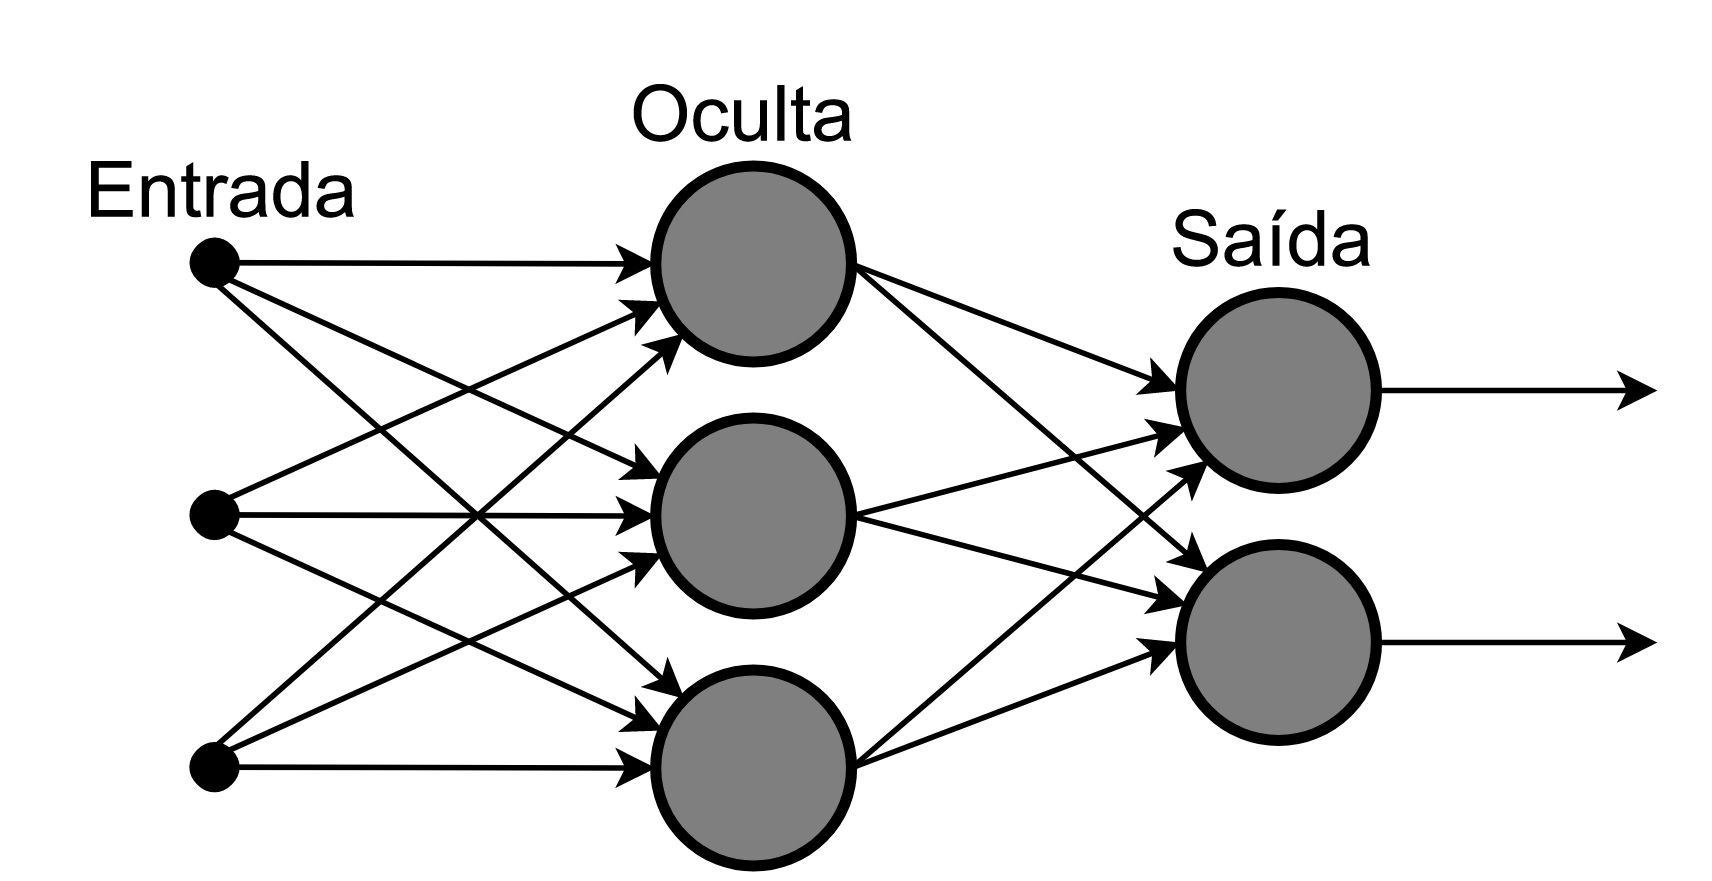
\includegraphics[scale=.25]{imagens/conceitos_basicos/artificial_neural_networks_arch.jpg}
    \label{fig:artificial_neural_networks_arch}
    \source{https://en.wikipedia.org/wiki/Artificial\_neural\_network}
\end{figure}

Na Figura \ref{fig:artificial_neural_networks_arch}, é introduzido uma rede neural \textit{feedforward} simples de três camadas, composta por uma camada de entrada (\textit{input}), uma camada oculta (\textit{hidden}) e uma camada de saída (\textit{output}). Essa estrutura é a base de uma série de arquiteturas comuns de ANN \cite{o2015introduction}.

A entrada é carregada geralmente na forma de um vetor multidimensional que será distribuída para as camadas ocultas da rede \cite{o2015introduction}. As camadas ocultas tomarão decisões a partir da camada anterior e avaliarão como uma mudança estocástica em si mesma avaliando se o resultado prejudica ou melhora o valor final obtido, e isso é conhecido como o processo de aprendizagem \cite{o2015introduction}. 

Existem diversas ramificações para determinação de um modelo de classificação para as redes neurais artificiais, normalmente os dois mais utilizados são aprendizado supervisionado e aprendizado não supervisionado.

\section{Redes neurais convolucionais}
Segundo \cite{yamashita2018convolutional}, as redes neurais convolucionais (CNN) são um tipo de modelo de aprendizado profundo para processamento de dados, inspiradas na organização do córtex visual animal e projetada para aprender de forma automática e adaptativa, hierarquias espaciais de recursos disponíveis em imagens digitais de padrões de baixo a alto nível. A CNN normalmente é composta de três tipos de camadas, convolução (\textit{convolutional layer}), agrupamento (\textit{pooling layer}) e camadas totalmente conectadas (\textit{fully-connected layer}) conforme o exemplo apresentado na Figura \ref{fig:arquitetura_cnn_mnist}.

\begin{figure}[H]
    \centering
    \caption{Constituição macro de uma CNN}
    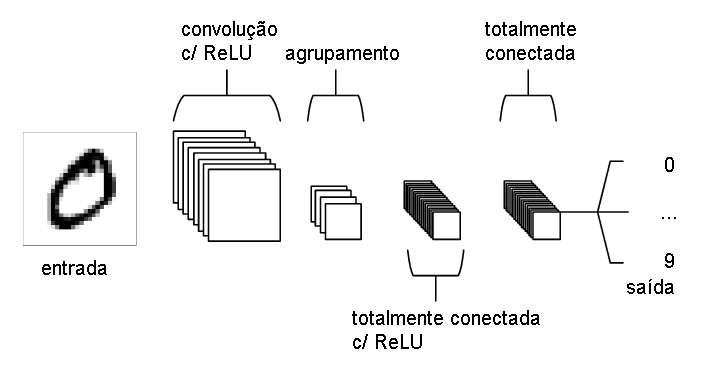
\includegraphics[scale=.65]{imagens/conceitos_basicos/arquitetura_cnn_mnist.jpg}
    \label{fig:arquitetura_cnn_mnist}
    \source{\citeonline{o2015introduction}}
\end{figure}

As camadas de convolução e agrupamento executam a extração de recursos, enquanto a camadas totalmente conectada mapeia os recursos extraídos na saída final, como a classificação.

\subsection{Camada de convolução}
A camada de convolução (\textit{convolutional layer}) é um componente fundamental da arquitetura de uma CNN, tendo como objetivo a extração de recursos de uma imagem digital, que consiste normalmente em uma combinação de operações lineares e não lineares, ou seja, operação de convolução e função de ativação \cite{yamashita2018convolutional}.

Convolução é um tipo especializado de operação linear, usado para o processo de extração de recursos onde um filtro (\textit{kernel}) é aplicada na entrada que é uma matriz de números, chamada de \textit{tensor} \cite{o2015introduction}. Estes filtros são geralmente pequenos em dimensionalidade espacial, mas se espalham ao longo de toda a profundidade da entrada \cite{o2015introduction}. Quando os dados atingem uma camada convolucional, a camada convolve cada filtro na dimensionalidade espacial da entrada, para assim produzir um mapa de ativação 2D (bidimensional) \cite{o2015introduction}. Conforme navegamos pela entrada, o produto escalar é calculado para cada valor naquele filtro, como é mostrado na Figura \ref{fig:convolution_cnn}. A partir disso, a rede aprenderá os filtros que são excitados quando veem um recurso específico em uma determinada posição espacial da entrada. Esses são comumente conhecidos como ativações \cite{o2015introduction}.

\begin{figure}[H]
    \centering
    \caption{Processo da convolução em dados de entrada}
    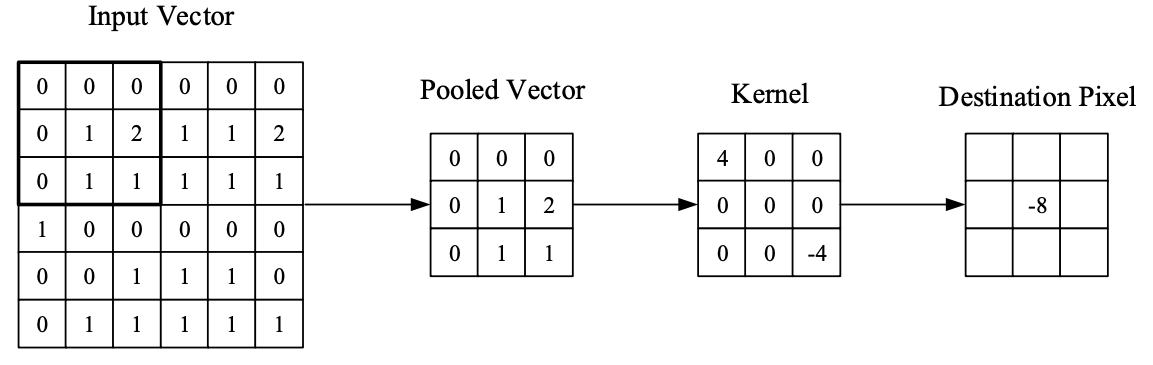
\includegraphics[scale=.35]{imagens/conceitos_basicos/convolution_cnn.png}
    \label{fig:convolution_cnn}
    \source{\citeonline{o2015introduction}}
\end{figure}

A operação de convolução descrita acima, não permite que o centro de cada filtro se sobreponha ao elemento mais externo do \textit{tensor} de entrada, e reduz a altura e largura do mapa de recursos de saída em comparação com o \textit{tensor} de entrada \cite{yamashita2018convolutional}.

Camadas convolucionais também são capazes de reduzir significativamente a complexidade do modelo por meio da otimização de sua saída. Eles são otimizados por meio de três hiperparâmetros, a profundidade (\textit{depth}), a passada (\textit{stride}) e a configuração de preenchimento (\textit{padding}) \cite{o2015introduction}. 

A profundidade (\textit{depth}) do volume de saída produzido pelas camadas convolucionais pode ser ajustada manualmente através do número de neurônios dentro da camada para a mesma região da entrada \cite{o2015introduction}. Isso pode ser visto com outras formas de ANNs, onde todos os neurônios na camada oculta são conectados diretamente a cada neurônio de antemão \cite{o2015introduction}. A redução desse hiperparâmetro pode minimizar significativamente o número total de neurônios da rede, mas também pode reduzir significativamente os recursos de reconhecimento de padrão do modelo \cite{o2015introduction}.

A passada (\textit{stride}) serve para definir a profundidade em torno da dimensionalidade espacial da entrada, e posicionar o campo receptivo \cite{o2015introduction}. Ou seja, se definíssemos uma passada como 1, conforme exibido na Figura \ref{fig:convolution_stride_cnn}, teríamos um forte campo receptivo sobreposto, produzindo ativações extremamente grandes \cite{o2015introduction}. Alternativamente, definir a passada para um número maior, reduzirá a quantidade de sobreposição e produzirá uma saída de dimensões espaciais menores \cite{o2015introduction}.

\begin{figure}[H]
    \centering
    \caption{Stride 1 no processo convolucional}
    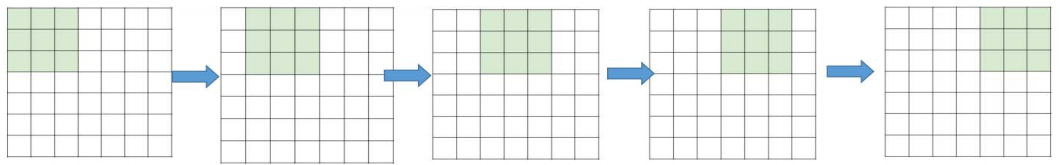
\includegraphics[scale=.40]{imagens/conceitos_basicos/convolution_stride_cnn.png}
    \label{fig:convolution_stride_cnn}
    \source{\citeonline{albawi2017understanding}}
\end{figure}

Preenchimento (\textit{Padding}), usualmente preenchimento de zero (\textit{zero padding}), é uma técnica onde linhas e colunas de zeros são adicionadas em cada lado do tensor de entrada, de modo a ajustar o centro de um filtro no elemento mais externo, e mantendo a mesma dimensão no plano através da operação de convolução \cite{yamashita2018convolutional}. As arquiteturas modernas de CNN geralmente empregam preenchimento zero, para assim reter as dimensões no plano e aplicar mais camadas \cite{yamashita2018convolutional}. Sem o preenchimento de zero, cada mapa de recurso sucessivo ficaria menor após a operação de convolução \cite{yamashita2018convolutional}.

\subsection{Função de ativação não linear}
As saídas de uma operação linear, como a convolução, são passadas por uma função de ativação não linear \cite{albawi2017understanding}. Embora funções não lineares, como a função sigmoide ou tangente hiperbólica (tanh), foram usadas anteriormente por serem representações matemáticas de um comportamento de neurônio biológico, a função de ativação mais comum usada atualmente é a unidade linear retificada (ReLU), devido sua facilidade em computar sua derivadas. A ReLu é expressada pela seguinte Fórmula \ref{equation_relu}:

\begin{equation}
  ReLU(x)=\max(0, x)
  \label{equation_relu}
\end{equation}

Ambas as funções não lineares citadas podem ser melhor observadas a partir da Figura \ref{fig:nonlinearity_functions}, onde é possível observar suas composições do ponto de vista gráfico.

\begin{figure}[H]
    \centering
    \caption{funções de ativação não lineares}
    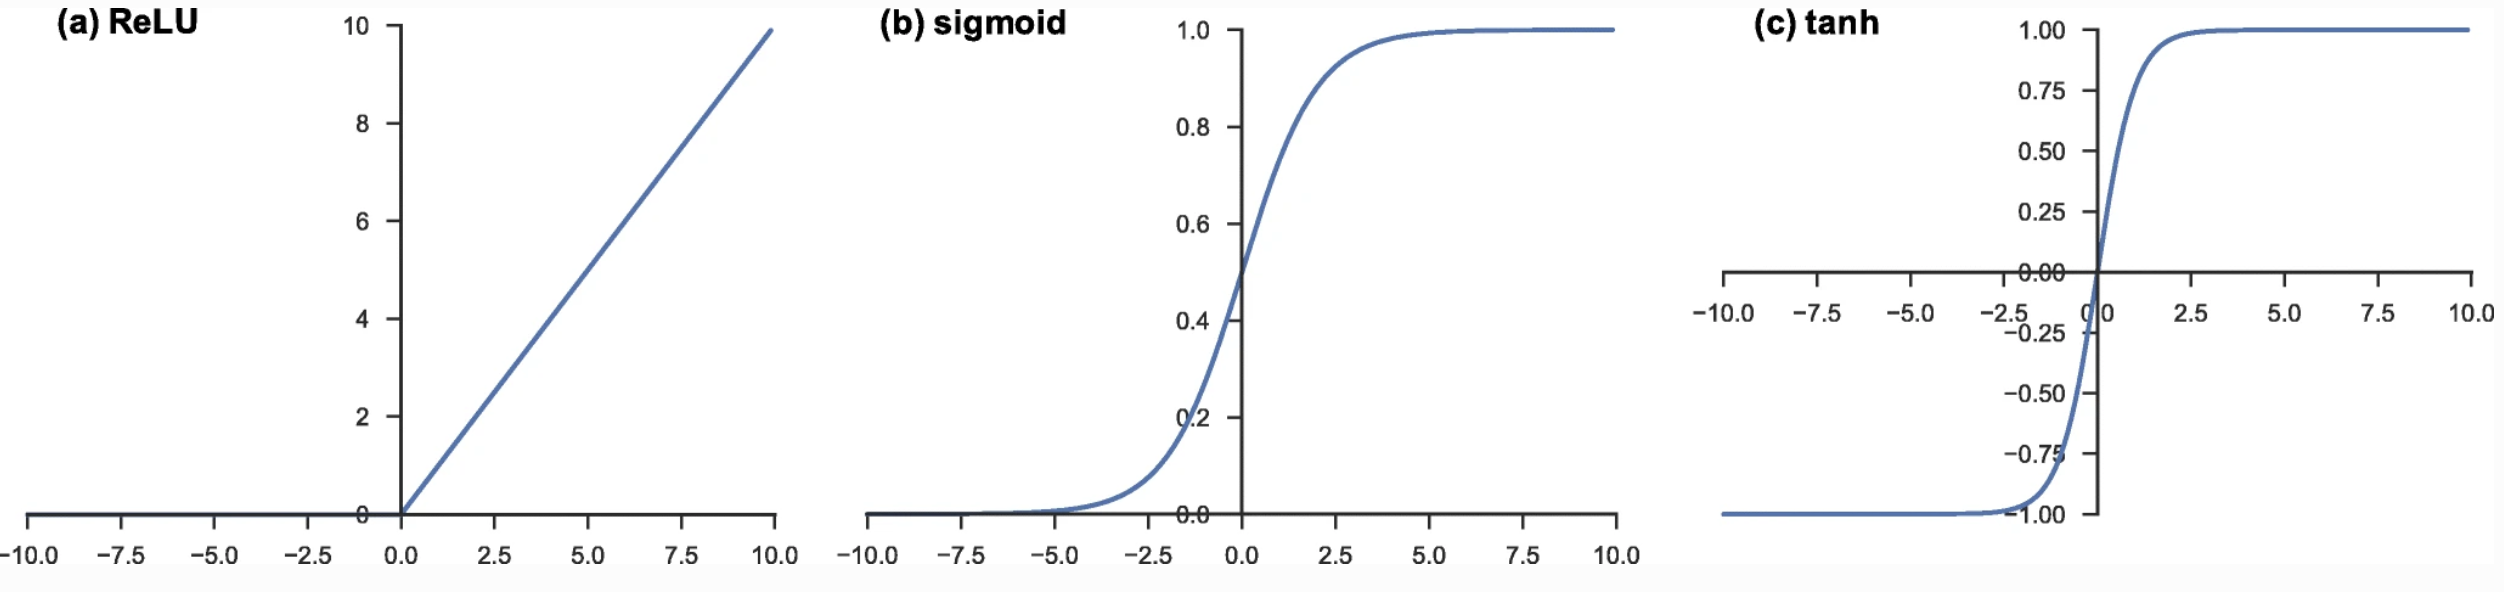
\includegraphics[scale=.35]{imagens/conceitos_basicos/nonlinearity_functions.png}
    \label{fig:nonlinearity_functions}
    \source{\citeonline{yamashita2018convolutional}}
\end{figure}

\subsection{Camada de agrupamento}
O objetivo da camada de agrupamento (\textit{pooling layer}) é transformar a representação de característica conjunta em uma mais utilizável, que preserve informações importantes enquanto descarta detalhes irrelevantes \cite{yu2014mixed}. Ou seja, a camada de agrupamento visa reduzir gradualmente a dimensionalidade da representação e, assim, reduzir ainda mais o número de parâmetros e complexidade computacional do modelo \cite{o2015introduction}. A operação oferecida pelo agrupamento é tipicamente conhecido como \textit{downsampling}. Devido a natureza presente no processo de agrupamento, um filtro com tamanho acima de 3 geralmente reduzirá muito o desempenho do modelo, portanto, na maioria das CNNs, filtros são configurados com dimensionalidade de 2 x 2 com passada de 2 na camada de agrupamento, o que permitirá que a camada se estenda por toda a dimensionalidade espacial da entrada recebida, reduzindo o mapa de ativação para 25\% do tamanho original enquanto é mantido o volume de profundidade em seu tamanho padrão \cite{yamashita2018convolutional}. É importante notar que não há nenhum parâmetro aprendível em nenhuma das camadas de agrupamento, enquanto o tamanho do filtro, a passada (\textit{stride}) e o preenchimento (\textit{padding}) são também hiperparâmetros em operações de agrupamento, semelhantes às operações de convolução \cite{yamashita2018convolutional}. A camada de agrupamento ajusta sua dimensionalidade usando uma função de agrupamento, podendo ser funções como a \textit{Max Pooling} ou \textit{Average Pooling}.

\textit{Max Pooling} é a forma mais popular de operação de agrupamento, que extrai \textit{patches} dos mapas de recursos de entrada, produz o valor máximo em cada \textit{patch} e descarta todos os outros valores \cite{yamashita2018convolutional}. O \textit{Max Pooling} com um filtro de tamanho 2 × 2 com uma passada de 2 é comumente usado na prática. Isso diminui a resolução da dimensão no plano dos mapas de recursos por um fator de 2, e, ao contrário da altura e da largura, a dimensão de profundidade dos mapas de recursos permanece inalterada \cite{yamashita2018convolutional}. Este método pode ser observado pela Figura \ref{fig:max_pooling}.

\begin{figure}[H]
    \centering
    \caption{funções de ativação não lineares}
    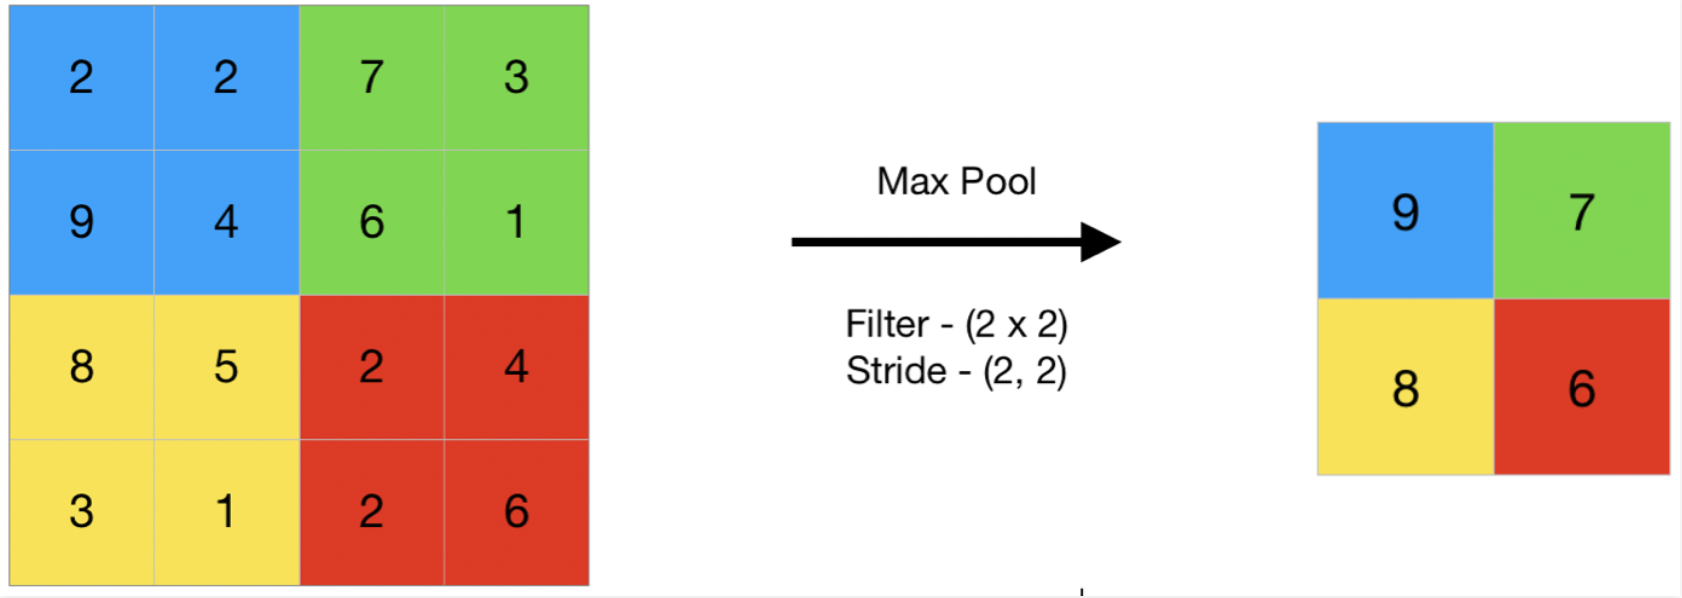
\includegraphics[scale=.45]{imagens/conceitos_basicos/max_pooling.png}
    \label{fig:max_pooling}
    \source{Danilo Assunção, 2021}
\end{figure}

O \textit{Average Pooling} extrai \textit{patches} dos mapas de recursos de entrada e calcula a média destes elementos. Assim, enquanto o \textit{Max Pooling} fornece o recurso mais proeminente em um \textit{patch} específico do mapa de recursos, o \textit{Average Pooling} fornece a média de recursos presentes em um \textit{patch}, conforme a Figura \ref{fig:average_pooling}.

\begin{figure}[H]
    \centering
    \caption{funções de ativação não lineares}
    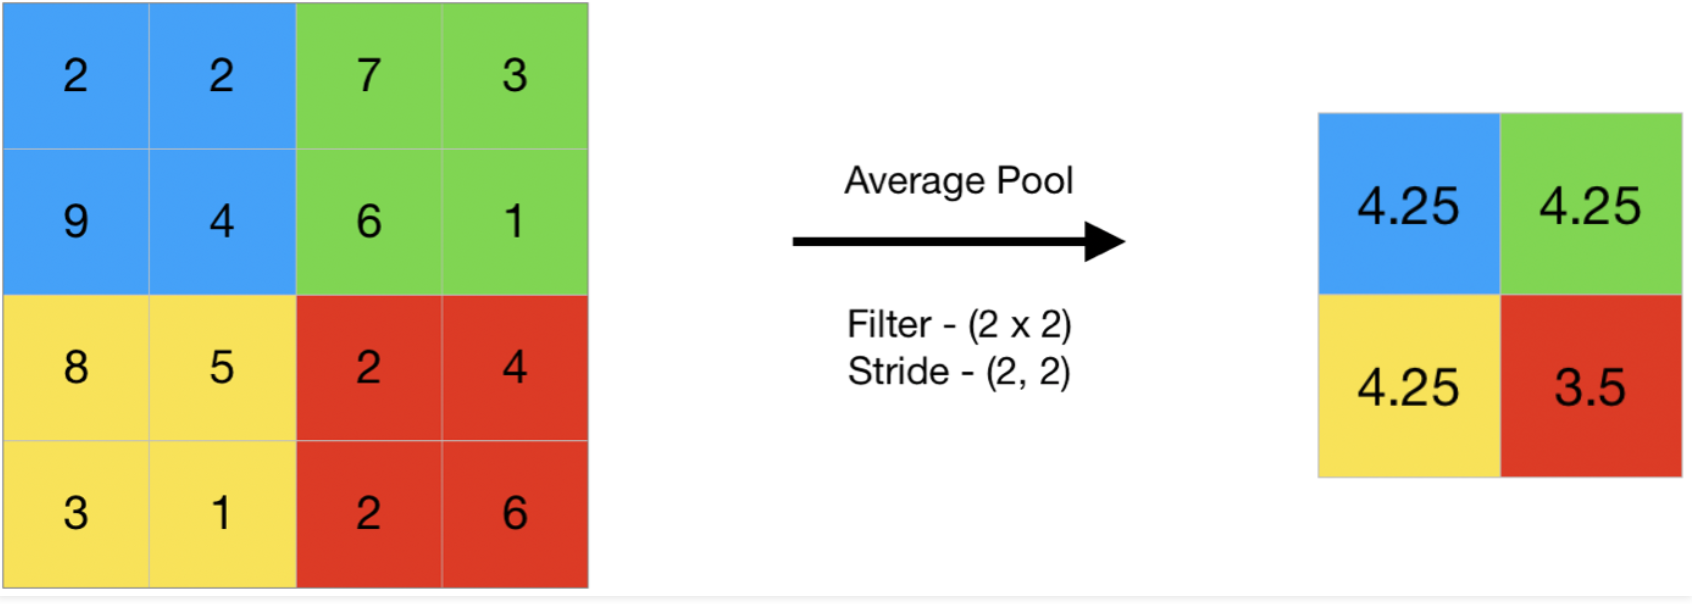
\includegraphics[scale=.45]{imagens/conceitos_basicos/average_pooling.png}
    \label{fig:average_pooling}
    \source{Danilo Assunção, 2021}
\end{figure}

\subsection{Camada totalmente conectada}
Os mapas de recursos de saída da convolução final ou camada de agrupamento, são normalmente achatados (\textit{flattened}), ou seja, transformados em uma matriz unidimensional de números (ou vetor) e conectados a uma ou mais camadas totalmente conectadas, também conhecidas como camadas densas, em que cada entrada é conectada a cada saída por um peso aprendível \cite{yamashita2018convolutional}. Ao passar pelas camadas de convolução e agrupamento, o conteúdo resultando deste processo anterior é mapeado por um subconjunto de camadas totalmente conectadas para as saídas finais da rede \cite{yamashita2018convolutional}. A camada final totalmente conectada normalmente tem o mesmo número de nós de saída que o número de classes. Cada camada totalmente conectada é seguida por uma função não linear \cite{yamashita2018convolutional}.

\section{Técnica de aprendizado por transferência}
Segundo \citeonline{shao2014transfer}, a técnica de aprendizado por transferência (\textit{transfer learning}) é um paradigma para evitar sobreajuste. O aprendizado por transferência funciona treinando uma rede em um elevado conjunto de dados, como \textit{ImageNet}, para então usar tais pesos como os pesos iniciais em uma nova tarefa de classificação. Normalmente, apenas os pesos nas camadas convolucionais da CNN pré-treinada são copiados, em vez de toda a rede. Sua eficácia é notada pois muitos conjuntos de dados de imagem compartilham características espaciais de baixo nível, que são melhor aprendidas com grandes quantidades de dados. O aprendizado por transferência possui dois métodos aplicáveis disponíveis na literatura, sendo eles, a transferência de características (\textit{feature learning}) e o ajuste fino (\textit{fine-tuning}).

\subsection{Transferência de características}
O método de transferência de características (\textit{feature learning}) é um processo de remoção das camadas totalmente conectadas de uma rede pré-treinada e ao mesmo tempo manter o restante da rede, cuja composição deste restante se dá em uma série de camadas de convolução e agrupamento, denominada base convolucional, funcionando como um extrator de recursos fixo \cite{li2017learning}. Nesse cenário, qualquer classificador de aprendizado de máquina podem ser adicionados no topo do extrator de recursos fixo, como exemplo as máquinas de vetores de suporte (SVM), florestas aleatórias (\textit{random forest}) e bem como as camadas totalmente conectadas usuais em CNNs, resultando em um processo de treinamento focado no classificador adicionado em um determinado conjunto de dados de interesse \cite{li2017learning}. Este mecanismo pode ser visto na Figura \ref{fig:fixed_features_extraction}.

\begin{figure}[H]
    \centering
    \caption{Método de transferência de características}
    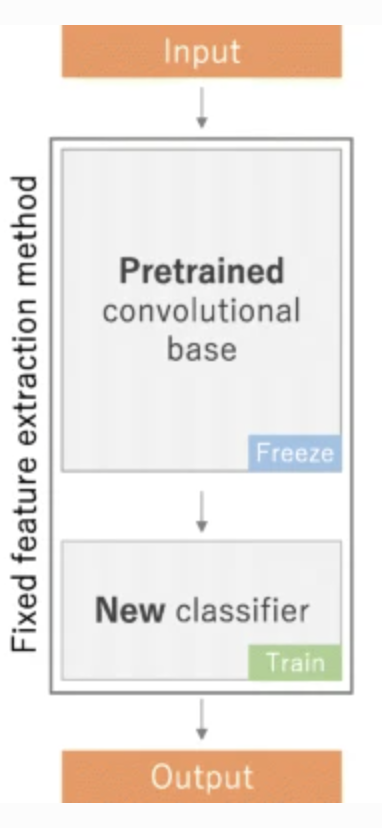
\includegraphics[scale=.55]{imagens/conceitos_basicos/fixed_features_extraction.png}
    \label{fig:fixed_features_extraction}
    \source{Danilo Assunção, 2021}
\end{figure}

\subsection{Ajuste fino}
O método de ajuste fino substitui as camadas totalmente conectadas do modelo pré-treinado por um novo conjunto de camadas totalmente conectadas para retreinar em um determinado conjunto de dados, aplicando também o ajuste fino como um todo ou apenas partes dos componentes na base convolucional pré-treinada \cite{li2017learning}. Todas as camadas na base convolucional podem ser ajustadas ou, alternativamente, algumas camadas anteriores podem ser corrigidas durante o ajuste fino do resto das camadas mais profundas \cite{li2017learning}. Isso é motivado pela observação de que os recursos da camada inicial terem um fator maior de generalização, enquanto os recursos posteriores tornam-se progressivamente mais específicos para um determinado conjunto de dados \cite{li2017learning}. Este mecanismo pode ser visto na Figura \ref{fig:fine_tuning_method}.

\begin{figure}[H]
    \centering
    \caption{Método de ajuste fino}
    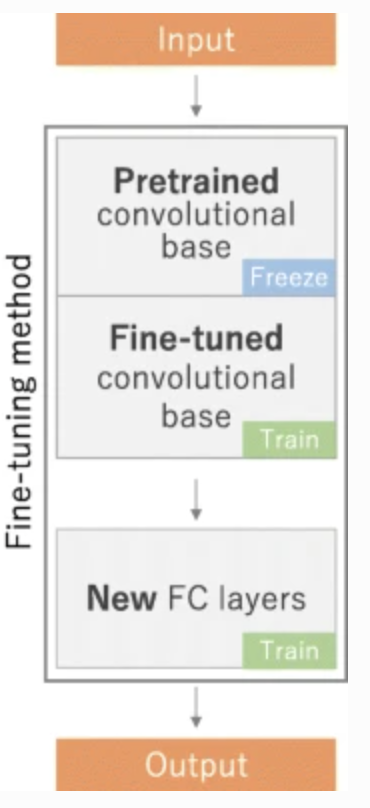
\includegraphics[scale=.55]{imagens/conceitos_basicos/fine_tuning_method.png}
    \label{fig:fine_tuning_method}
    \source{Danilo Assunção, 2021}
\end{figure}

\section{Técnica de aumento de dados}
Segundo \citeonline{shorten2019survey}, a técnica de aumento de dados (\textit{data augmentation}) abrange um conjunto de métodos que aumentam o tamanho dos conjuntos de dados de treinamento, nessa conformidade, melhores modelos de aprendizado profundo podem ser construídos com eles devido a sua capacidade em minimizar o sobreajuste. Os algoritmos de aumento de dados incluem transformações geométricas (\textit{geometric transformations}), modificação de espaço de cores (\textit{color space augmentations}), aplicação de máscara (\textit{kernel filters}), misturas de imagens (\textit{mixing images}), apagamento aleatório (\textit{random erasing}).

\subsection{Transformações geométricas}
Esta subseção descreve as diferentes metodologias com base em transformações geométricas aplicadas em imagens. Os tipos descritos abaixo podem ser caracterizados por sua facilidade de implementação \cite{shorten2019survey}. Estes mecanismos foram divididos em 6 partes principais:

\begin{enumerate}
  \item Inversão (\textit{Flipping}): o método de inversão consisti em em inverter o eixo horizontal ou vertical de uma imagem, onde a inversão do eixo horizontal costuma ser mais frequente do que a inversão do eixo vertical \cite{shorten2019survey}. Esta técnica é uma das mais simples de se implementar, e provou ser útil em determinados conjuntos de dados de imagens \cite{shorten2019survey}.
  
  \item Espaço dos canais de cores (\textit{Color space}): os dados de uma imagem digital são geralmente codificados como um tensor tridimensional (altura × largura × canais de cor), viabilizando a implementação de técnicas de aumento de dados no espaço de canais de cores \cite{shorten2019survey}. O método de espaço de cores inclui o isolamento de um simples canal de cor, tal como R, G ou B, sendo que, a imagem pode ter sua representação de cores rapidamente convertida ao isolar um canal de cor, e adicionando duas matrizes de zero nos demais canais \cite{shorten2019survey}. Adicionalmente, os valores nos canais de cores da imagem (RGB) podem ser manipulados com simples operações de matriz, ao aumentar ou diminuir o brilho da imagem.
  
  \item Corte (\textit{Cropping}): cortar imagens é uma prática de processamento onde áreas relevantes da imagem são destacadas e redimensionadas \cite{shorten2019survey}. Por exemplo, uma imagem de dimensão 256 x 256 onde, após o corte, ficou com dimensão 224 x 224. Dependendo do limite de redução escolhido para o corte, pode ser uma transformação que não preserve a classe que representa a imagem.
  
  \item Rotação (\textit{Rotation}): é a realização de rotação da imagem para a direita ou esquerda, em um eixo entre 1° e 359° \cite{shorten2019survey}. A segurança deste método é fortemente determinada pelo grau de rotação. Leves rotações entre 1 e 20 ou -1 a -20, podem ser úteis em tarefas de reconhecimento de dígitos, sendo que, à medida na qual o grau de rotação aumenta, a classe que representa os dados pode não mais ser preservada após aplicado tal transformação \cite{shorten2019survey}.
  
  \item Deslocamento (\textit{shifting}): é um método de deslocação de imagens para a esquerda, direita, cima ou baixo, podendo ser uma transformação muito útil para evitar um viés no modelo e preservando as dimensões da imagem \cite{shorten2019survey}. Por exemplo, se todas as imagens em um conjunto de dados estiverem centralizadas, o que é comum em conjuntos de dados de reconhecimento de rosto, exigiria que o modelo também fosse testado em imagens perfeitamente centradas. Como a imagem original foi deslocada para um direção, o espaço restante pode ser preenchido com um valor constante, no caso de um modelo na escala RGB, seria aplicada a cor preta (0, 0, 0) ou a cor branca (255, 255, 255), ou então com ruído aleatório ou gaussiano \cite{shorten2019survey}.
  
  \item Injeção de ruído (\textit{Noise injection}): A injeção de ruído consiste em injetar uma matriz de valores aleatórios, normalmente extraídos de uma distribuição gaussiana. Adicionar ruído às imagens pode ajudar uma CNN a aprender recursos mais robustos \cite{shorten2019survey}.
\end{enumerate}

\subsection{Transformações fotométricas}
O canal de cores de uma imagem é composta por três matrizes bidimensionais empilhadas. Essas matrizes representam a cor RGB de um \textit{pixel}. O enviesamento de iluminação está entre os desafios que ocorrem com mais frequência aos problemas de reconhecimento de imagem \cite{shorten2019survey}. Uma solução para imagens excessivamente claras ou escuras é percorrer as imagens e diminuir ou aumentar os valores da matriz de cores dos \textit{pixels} aplicando uma determinada constante \cite{shorten2019survey}.

\subsection{Aplicação de máscara}
A aplicação de máscara, muito popular no processamento de imagens, é uma técnica que torna imagens mais nítidas ou desfocadas. Essas máscaras funcionam deslizando uma matriz bidimensional através de uma imagem com um filtro de desfoque Gaussiano, resultando em uma imagem mais desfocada ou um filtro de borda vertical ou horizontal de alto contraste, que resultará em uma imagem mais nítida ao longo das bordas \cite{shorten2019survey}. Intuitivamente, desfocar imagens para aumento de dados pode levar a uma maior resistência na classificação da imagem pelo modelo de aprendizado de máquina. Além disso, aumentar a nitidez de imagens para aumento de dados pode resultar no ocultamento de mais detalhes sobre regiões de interesse da imagem \cite{shorten2019survey}.

\subsection{Mistura de imagens}
Misturar imagens aplicando a média de seus valores de \textit{pixel} é uma abordagem muito contra-intuitiva para o aumento de dados. As imagens produzidas com isso não parecerão uma transformação útil para um observador humano, sendo que, o emparelhamento de amostras pode ser desenvolvido em uma estratégia de aumento eficaz \cite{shorten2019survey}. Neste experimento, duas imagens são cortadas aleatoriamente de 256 × 256 a 224 × 224, e invertidas aleatoriamente na horizontal. Essas imagens são então misturadas calculando a média dos valores de \textit{pixel} para cada um dos canais RGB \cite{shorten2019survey}. Isso resulta em uma imagem mista que é usada para treinar um modelo de classificação. O rótulo atribuído à nova imagem é o mesmo da primeira imagem selecionada aleatoriamente \cite{shorten2019survey}.

\subsection{Apagamento aleatório}
O apagamento aleatório é inspirada nos mecanismos de regularização de \textit{dropout} \cite{shorten2019survey}. \textit{Dropout} é uma técnica de regularização para reduzir o sobreajuste. Esta técnica foi projetada especificamente para combater os desafios de reconhecimento de imagem devido à oclusão \cite{shorten2019survey}. Oclusão (\textit{Occlusion}) se refere a algumas partes do objeto em uma imagem que não estão claras. O apagamento aleatório interromperá isso, forçando o modelo a aprender mais recursos descritivos sobre uma imagem, e evitando que ele se ajuste a um determinado recurso visual da imagem \cite{shorten2019survey}.

\section{Conclusão}
Neste capítulo foi introduzido uma série de conceitos importantes que estão amplamente relacionados a este trabalho de pesquisa, que envolve a aplicação de Redes Neurais Convolucionais (CNN) na resolução de cenários de reconhecimento de espécies. Contudo, a explicação para os conceitos de aprendizado de máquina e suas ramificações de mais baixo nível, como aprendizado profundo e CNN foram todas especificadas nesta seção, afim de constituir uma maior compreensão de todos os conceitos que estão sendo abrangidos nos próximos capítulos.

% ----------------------------------------------------------
% CAPITULO - REVISÃO SISTEMÁTICA
% ----------------------------------------------------------
\chapter{Revisão sistemática}
A revisão sistemática possibilita uma forma de analise e instrução a partir das informações dispostas pelos artigos disponíveis para uma pesquisa em especifico, assunto de tópico ou tema de interesse, sendo que deve ser utilizada uma sistemática de confiança, auditável e integra. \cite{garcia2020guidelines}.
O desenvolvimento da revisão sistemática se baseia em um protocolo devidamente definido para assim trazer resultados válidos e detalhados, trazendo assim a possibilidade de análise e contradição destes resultados a partir do uso do protocolo determinado.

\section{Objetivos da revisão}
Na área de visão computacional há a aplicação de técnicas com objetivo de identificação de insetos, onde a técnica de processamento baseado em imagens e algoritmos que reconhecem padrões e classificam assim, automaticamente as espécies de insetos. Tal processamento vem modificando o tradicional modelo manual e descritivo de características morfológicas já fornecido por estudos taxonômicos para a identificação destes insetos. Sendo que, apenas especialistas como taxonomistas e técnicos qualificados podem identificar tais insetos com precisão, pois isso requer conhecimento especializado e obtido por meio de uma vasta experiência \cite{lim2017performance}.
O aprendizado profundo tem sido amplamente utilizado em processamento de imagens, visão computacional e reconhecimento de padrões. Diferente dos métodos tradicionais de aprendizado de máquina, o modelo de aprendizado profundo pode aprender recursos automaticamente a partir de uma grande quantidade de imagens, e não requer um especialista com domínio na construção do extrator de características. \cite{liu2020classification}.

As características extraídas das imagens são os fatores que mais influenciam na acurácia do classificador. Embora existam várias técnicas e ferramentas para extração de características automaticamente, ainda não se encontram trabalhos na literatura que avaliem estas técnicas de aprendizado profundo e nem ferramentas que as entreguem de forma sistemática.

Portanto, o objetivo desta revisão sistemática é apresentar e discutir o estado da arte das técnicas de reconhecimento automático de espécies por meio de suas imagens e morfologias diversas, empregando técnicas de aprendizado profundo. Visando tal objetivo, foram analisados os artigos com foco na aplicação de Redes Neurais Convolucionais (CNN).

\section{Protocolo}

Foi coordenada em quatro fases para a realização desta revisão sistemática, sendo elas:

\begin{enumerate}
  \item Planejamento
  \item Condução
  \item Extração
  \item Consolidação
\end{enumerate}

O planejamento consiste na criação do protocolo no qual as diretrizes da pesquisa serão baseadas. A condução é a execução da pesquisa e seleção de trabalhos de interesse, de acordo com os critérios de inclusão e exclusão definidos do protocolo. A extração é a fase na qual os artigos que foram selecionados são estudados e os dados importantes são separados. Em suma, temos a consolidação, na qual os dados são cruzados para gerar conhecimento e , assim, o artigo de revisão sistemática é escrito.

A fase de planejamento é a determinação dos critérios de pesquisa para a formulação do protocolo. Na fase de condução é realizada a pesquisa de trabalhos, seguido da inclusão e exclusão destes trabalhos a partir dos itens baseados no protocolo. Já na fase de extração ocorre o estudo e a separação de dados importantes extraídos dos trabalhos selecionados. Por fim a fase de consolidação, onde é realizada a comparação entre os dados obtidos para o ganho de ciência, e seguidamente criar um artigo de revisão sistemática.

Estes processos estão representados na Figura \ref{fig:processo_revisao_sistematica}, na qual cada etapa do processo estão identificados com uma cor diferente.

\begin{figure}[H]
    \centering
    \caption{Diagrama do processo de revisão sistemática}
    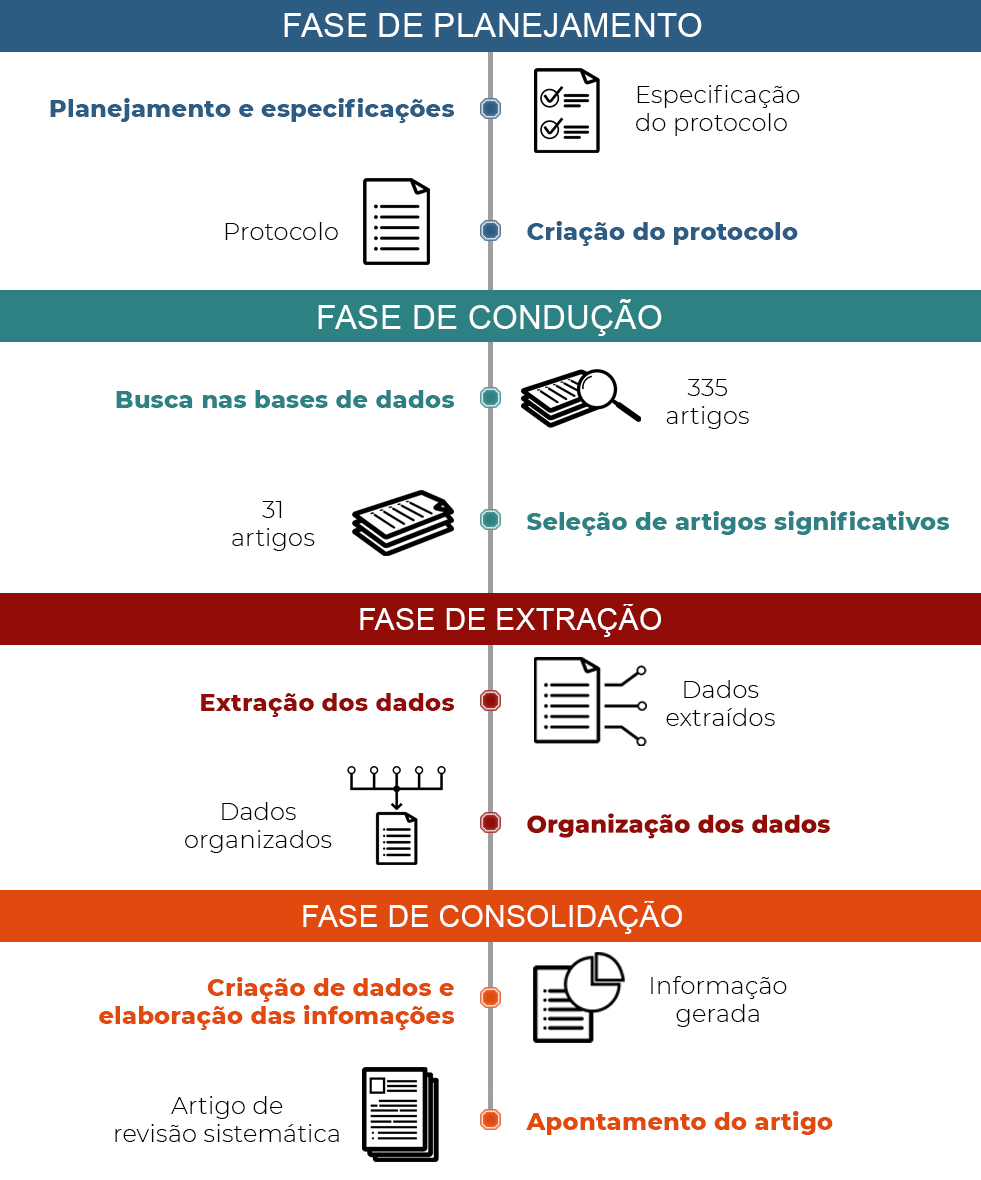
\includegraphics[scale=.35]{imagens/revisao_sistematica/processo_revisao_sistematica.jpg}
    \label{fig:processo_revisao_sistematica}
    \source{Danilo Assunção, 2021}
\end{figure}

Na etapa de planejamento foi levantada junto ao protocolo a distinta questão:
``Quais são os métodos que sejam o estado da arte, para identificação de espécies utilizando Redes Neurais Convolucionais por meio de imagens digitais?''.
A conclusão desta pergunta veio a partir de bases de dados junto às seguintes \textit{strings} de busca:

\begin{itemize}
  \item \textbf{IEEE Xplore} - (``convolutional neural network'' OR ``cnn'' OR ``convolution'') AND ``feature extraction'' AND (``insect'' OR ``pest'') AND (``image'' OR ``image segmentation'' OR ``image recognition'')
  \item \textbf{SCOPUS} - (``convolutional neural network'' OR ``cnn'' OR ``convolution'') AND ``feature extraction'' AND (``insect'' OR ``pest'') AND (``image'' OR ``image segmentation'' OR ``image recognition'') AND (EXCLUDE (DOCTYPE, ``cp'') OR EXCLUDE (DOCTYPE, ``re'') OR EXCLUDE (DOCTYPE, ``bk'') OR EXCLUDE (DOCTYPE, ``ch''))
\end{itemize}

A palavra chave \textit{pest} é incluída nas \textit{strings} de busca por se tratar de um objeto de estudo muito recorrente nos meios de reconhecimento de espécies através de imagens, utilizando de técnicas similares às que são usadas para reconhecimento de insetos por meio de métodos utilizando CNN.

Este trabalho foi conduzido de dezembro de 2020 até fevereiro de 2021. Inicialmente 335 trabalhos foram encontrados nas bases de dados especificadas acima, dos quais 302 estavam na base de dados SCOPUS e 33 na base de dados IEEE Xplore.

Após aplicar os critérios de inclusão e exclusão nos trabalhos coletados, 31 artigos foram selecionados e analisados por completo, sendo 28 da base SCOPUS e 3 da base IEEE Xplore.

Os critérios utilizados para incluir ou excluir um trabalho nesta revisão foram:

\begin{itemize}
  \item Inclusão
    \begin{itemize}
        \item{Artigos que utilizam Redes Neurais Convolucionais como ferramenta para discriminação de espécies por meio de imagens digitais;}
        \item{Artigos que contém técnicas computacionais de segmentação e extração de características de imagens digitais de diversas espécies biológicas;}
        \item{Artigos devem ter data de publicação maior ou igual a 2015.}
    \end{itemize}
  \item Exclusão
    \begin{itemize}
        \item{Artigos que não são relacionados com conceitos envolvendo técnicas de segmentação e extração de características por meio de imagens digitais;}
        \item{Artigos que não utilizam Redes Neurais Convolucionais para classificação automática de espécies por meio de imagens digitais;}
        \item{Artigos que não foram escritos com o idioma inglês ou português;}
        \item{Artigos com data de publicação menor que 2015;}
        \item{Documentos que não estejam categorizados como artigo em seu tipo de documento.}
    \end{itemize}
\end{itemize}

De cada trabalho selecionado foram extraídos tais atributos como, Ano de publicação, País de afiliação dos autores, Técnicas de pré-processamento de imagens, Técnica de aprendizado por transferência, Técnicas de aumento de dados, Modelo de arquitetura da CNN e Modelo do classificador.

Com a finalidade de poder encontrar possíveis lapsos nas pesquisas utilizadas, seguidamente da extração de dados, foi exercida uma averiguação sobre os principais obstáculos e propensões praticadas.

\section{Resultado da revisão sistemática}
Os 31 trabalhos selecionados foram estudados e os seguintes atributos foram extraídos: técnica de extração de características, tipos de características extraídas, principal país de afiliação dos pesquisadores e ano de publicação. Um breve sumário dos trabalhos com os respectivos dados extraídos encontram-se no Tabela \ref{tab:sumario_artigos_selecionados}.

% -----------------------------------------
% TABELA - SUMÁRIO DOS ARTIGOS ANALISADOS
% -----------------------------------------
\begin{landscape}
\begin{OnehalfSpacing}
\begin{footnotesize}
\begin{longtable}{|p{2.3cm}|p{1.3cm}|p{2cm}|p{2.6cm}|p{2.4cm}|p{4.3cm}|p{4.3cm}|p{2.5cm}|}
\caption{Sumário de todos os artigos analisados} \label{tab:sumario_artigos_selecionados} \\

\hline \textbf{Artigo} &
  \textbf{Ano de publicação} &
  \textbf{País de afiliação dos autores} &
  \textbf{Téc. de pré- processamento de imagens} &
  \textbf{Téc. de aprendizado por transferência} &
  \textbf{Téc. de aumento de dados} &
  \textbf{Modelo de arquitetura da CNN} &
  \textbf{Modelo do classificador} \\ \hline
\endfirsthead

\multicolumn{8}{c}%
{{\bfseries \tablename\ \thetable{} -- continuação da página anterior}} \\
\hline \textbf{Artigo} &
  \textbf{Ano de publicação} &
  \textbf{País de afiliação dos autores} &
  \textbf{Téc. de pré- processamento de imagens} &
  \textbf{Téc. de aprendizado por transferência} &
  \textbf{Téc. de aumento de dados} &
  \textbf{Modelo de arquitetura da CNN} &
  \textbf{Modelo do classificador} \\ \hline
\endhead

\hline \multicolumn{8}{|r|}{{Continua na próxima página}} \\ \hline
\endfoot

\hline \multicolumn{8}{|c|}{Fonte - Danilo Assunção, 2021} \\ \hline
\endlastfoot

\cite{liu2020classification} &
  2020 &
  Estados Unidos &
  Não aplicado &
  Fine-tuning &
  Skewing, Elastic distortion, Rotation &
  LeNet-5, AlexNet, VGGNet-16, VGGNet-19, ResNet-50, Inception v3, InceptionResNet v2 &
  Camada totalmente conectada \\ \hline
\cite{le2020automated} &
  2020 &
  França & 
  Resize &
  Fine-tuning &
  Constant to each channel, Split the channels of image &
  EB-Net &
  Camada totalmente conectada \\ \hline
\cite{zhangautomatic} &
  2020 &
  China &
  Não especificado &
  Não especificado &
  Não especificado &
  DenseNet-121 &
  Não especificado \\ \hline
\cite{liu2020grape} &
  2020 &
  China &
  Não aplicado &
  Não aplicado &
  High brightness, Low brightness, High contrast, Low contrast, High sharpness, Low sharpness, Rotation, Vertical symmetry, Horizontal symmetry, Gaussian noise, PCA Jittering &
  DICNN &
  Camada totalmente conectada \\ \hline
\cite{lu2020identifying} &
  2020 &
  Taiwan &
  Resize &
  Fine-tuning &
  Horizontal flipping, Vertical flipping, Width shifting, Height shifting, Rotation, Shearing, Zooming &
  VGGNet-16 &
  Camada totalmente conectada \\ \hline
\cite{banan2020deep} &
  2020 &
  Irã &
  Resize &
  Fine-tuning &
  Rotation, Height shifting, Width shifting &
  VGGNet-16 &
  Camada totalmente conectada \\ \hline
\cite{tiwari2020comparative} &
  2020 &
  India &
  Não especificado &
  Não aplicado &
  Não aplicado &
  CNN &
  Camada totalmente conectada \\ \hline
\cite{li2020using} &
  2020 &
  China &
  Cropping, Resize &
  Não aplicado &
  Rotation, Clipping &
  VGGNet-16, Inception v3 &
  Camada totalmente conectada \\ \hline
\cite{chen2020research} &
  2020 &
  China &
  Resize &
  Fine-tuning &
  Rotation, Blurred, Occluded &
  ResNeXt-101 &
  Camada totalmente conectada \\ \hline
\cite{hongclassification} &
  2020 &
  China &
  Resize, Cropping &
  Fine-tuning &
  Gaussian filter, Contrast enhancement &
  AlexNet &
  Camada totalmente conectada \\ \hline
\cite{rauf2019visual} &
  2019 &
  Paquistão, Estados Unidos &
  Resize, Transparent background &
  Não aplicado &
  Não aplicado &
  32-Layer CNN &
  Camada totalmente conectada \\ \hline
\cite{gomez2019coral} &
  2019 &
  Espanha, Dinamarca &
  Não especificado &
  Fine-tuning &
  Não especificado &
  Inception v3, ResNet-50, ResNet-152, DenseNet-121, DenseNet-161 &
  Camada totalmente conectada \\ \hline
\cite{cibuk2019efficient} &
  2019 &
  Turquia, Estados Unidos &
  Não aplicado &
  Feature transfer &
  Não aplicado &
  VGGNet-16, AlexNet &
  SVM (Kernel RBF) \\ \hline
\cite{li2019effective} &
  2019 &
  China &
  Resize &
  Não aplicado &
  Multi-scale, Rotation &
  ResNet-50 &
  Camada totalmente conectada \\ \hline
\cite{khalifa2019deep} &
  2019 &
  Egito, Luxemburgo &
  Não especificado &
  Não aplicado &
  Reflection, Zooming, Gaussian noise, Poisson noise, Salt and pepper noise, Speckle noise &
  CNN &
  Camada totalmente conectada \\ \hline
\cite{hsiang2019endless} &
  2019 &
  Suécia, Reino Unido &
  Resize &
  Fine-tuning &
  Não especificado &
  VGGNet-16, DenseNet-121, Inception v3 &
  Camada totalmente conectada \\ \hline
\cite{ren2019feature} &
  2019 &
  Japão &
  Resize, Cropping &
  Não aplicado &
  Resize, Cropping, Mean and standard deviation normalization &
  FR-ResNet &
  Camada totalmente conectada \\ \hline
\cite{valan2019automated} &
  2019 &
  Suécia &
  Resize, Cropping &
  Feature transfer &
  Não aplicado &
  VGGNet-16 &
  SVM (Kernel Linear) \\ \hline
\cite{gyires2019deep} &
  2019 &
  Hungria &
  Cropping, Resize &
  Fine-tuning &
  Não aplicado &
  AlexNet, Inception V3 &
  Camada totalmente conectada \\ \hline
\cite{thenmozhi2019crop} &
  2019 &
  India &
  Gray scale, Canny Edge Detection, Cropping, Resize &
  Fine-tuning &
  Reflection, Scaling, Rotation, Translation &
  VGGNet-16, VGGNet-19 &
  Camada totalmente conectada \\ \hline
\cite{tetila2019deep} &
  2019 &
  Brasil &
  Não especificado &
  Fine-tuning, Feature transfer &
  Rotation, Scaling, Scrolling, Zooming &
  DenseNet-201, InceptionResNet v2, ResNet-50 &
  Camada totalmente conectada \\ \hline
\cite{wei2018deep} &
  2018 &
  Malasia &
  Resize, Padding &
  Não aplicado &
  Não aplicado &
  D-Leaf &
  Camada totalmente conectada \\ \hline
\cite{zhu2018method} &
  2018 &
  China &
  Não especificado &
  Não aplicado &
  Não aplicado &
  Inception v2 &
  Camada totalmente conectada \\ \hline
\cite{zhu2018plant} &
  2018 &
  China &
  Resize &
  Não especificado &
  Não aplicado &
  CNN &
  SVM (Kernel Linear) \\ \hline
\cite{villon2018deep} &
  2018 &
  França &
  Não especificado &
  Não aplicado &
  Não aplicado &
  GoogLeNet &
  Camada totalmente conectada \\ \hline
\cite{lee2017deep} &
  2017 &
  Malásia, Reino Unido &
  Resize &
  Fine-tuning &
  Rotation &
  CNN &
  Camada totalmente conectada \\ \hline
\cite{zielinski2017deep} &
  2017 &
  Polônia &
  Não especificado &
  Feature transfer &
  Não aplicado &
  AlexNet, VGGNet-M, VGGNet-VD &
  SVM (Kernel Linear, RBF e Polinomial), Random Forest \\ \hline
\cite{wang2017crop} &
  2017 &
  China &
  Não especificado &
  Não especificado &
  Não aplicado &
  LeNet-5, AlexNet &
  Camada totalmente conectada \\ \hline
\cite{lim2017performance} &
  2017 &
  Coreia do Sul &
  Resize, Cropping &
  Não especificado &
  Rotation, Zooming &
  AlexNet &
  Camada totalmente conectada \\ \hline
\cite{sun2017deep} &
  2017 &
  China &
  Não especificado &
  Não aplicado &
  Não aplicado &
  ResNet-26 &
  Camada totalmente conectada \\ \hline
  
\end{longtable}
\end{footnotesize}
\end{OnehalfSpacing}
\end{landscape}

\subsection{Ano de publicação}
Nesta revisão sistemática foi coletado o ano de publicação dos artigos, dessa maneira, fez-se  uma análise de tendência referente aos assuntos que abordam técnicas de reconhecimento de espécies utilizando redes neurais convolucionais, em domínios que envolvem assuntos relacionados à reconhecimento de espécies.

Visando uma melhor compreensão sobre a quantidade de publicações com base em assuntos que envolvem reconhecimento automático de espécies utilizando técnicas de aprendizado profundo, foi elaborado um gráfico com todos os artigos encontrados na base de dados pela consulta feita nas bases do SCOPUS e IEEE Xplore. 

Na Figura \ref{fig:grafico_ano_vs_quantidade} é apresentado uma linha de tendência aos assuntos envolvendo artigos que possuem as palavras chaves, aprendizado profundo, redes neurais convolucionais e reconhecimento de espécies.

\begin{figure}[H]
    \centering
    \caption{Ano de publicação dos artigos com base em palavras chaves}
    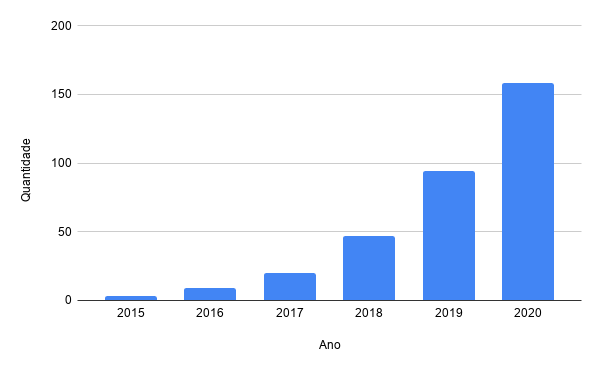
\includegraphics[scale=.60]{imagens/revisao_sistematica/grafico_ano_vs_quantidade.png}
    \label{fig:grafico_ano_vs_quantidade}
    \source{Danilo Assunção, 2021}
\end{figure}

Na Figura \ref{fig:grafico_ano_vs_publicacao} é demonstrado uma relação de quantidade versus ano, para o total de artigos que foram filtrados e selecionados a partir do conjunto obtido nas consultas executadas nas bases do SCOPUS e IEEE Xplore para esta revisão sistemática.

\begin{figure}[H]
    \centering
    \caption{Ano de publicação dos artigos selecionados}
    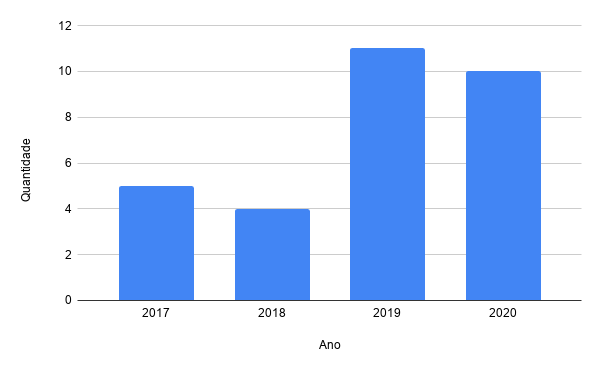
\includegraphics[scale=.60]{imagens/revisao_sistematica/grafico_ano_vs_publicacao.png}
    \label{fig:grafico_ano_vs_publicacao}
    \source{Danilo Assunção, 2021}
\end{figure}

Nota-se que a maior quantidade dos artigos selecionados foram publicados em 2019, representando um total de 36,67\% (11). Já em 2020, é tido 33,33\% (10) dos artigos. Em 2018 a quantia de artigos foi de 13,33\% (4) e em 2017, 16,67\% (5).

É possível perceber que, desde 2017 até 2020, houve um aumento significativo de artigos de interesse publicados com relação à aplicação de redes neurais convolucionais que almejam a resolução de problemas envolvendo reconhecimento de espécies em imagens digitais. Essa representatividade demonstra a veracidade de uma tendência de alta, com relação à utilização de técnicas envolvendo redes neurais convolucionais neste tipo de aplicação \cite{liu2020classification}.

Os artigos de interesse obtidos possuem data de publicação a partir do ano de 2017, os artigos de 2015 a 2016 não se mostraram muito relevantes para os assuntos relacionados à esta revisão sistemática, sendo levado em consideração os critérios de exclusão definidos.

\subsection{País de afiliação dos autores}
Foi feito a extração de dados sobre os países de cada pesquisador contribuinte em determinado artigo e esta visão pode ser na partir da Figura \ref{fig:grafico_pais_vs_publicacao}.

\begin{figure}[H]
    \centering
    \caption{País de afiliação dos pesquisadores}
    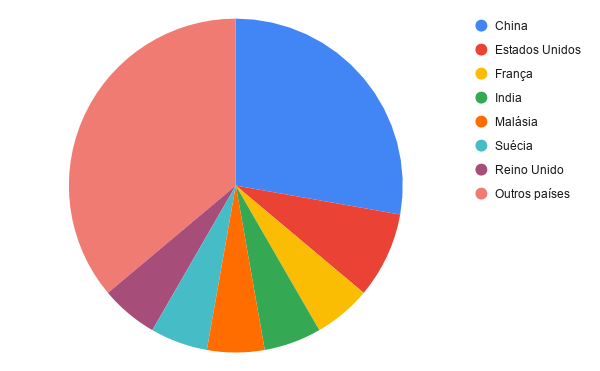
\includegraphics[scale=.60]{imagens/revisao_sistematica/grafico_pais_vs_publicacao.png}
    \label{fig:grafico_pais_vs_publicacao}
    \source{Danilo Assunção, 2021}
\end{figure}

Pode ser visto que, com base nos artigos selecionados, a China possui a liderança com relação à produção de artigos científicos relacionados a identificação e classificação de espécies por meio do uso de Redes Neurais Convolucionais, possuindo 27,78\% (10 artigos) em relação aos pesquisadores de outros países. Os Estados Unidos, em segundo colocado, possuindo 8,33\% (3 artigos). A França, Índia, Malásia, Suécia e o Reino Unido possuem ambos 5,56\% (2 artigos) artigos publicados. Já na categoria ``Outros países'', que compõe os 36,11\% dos artigos publicados restantes, são as demais regiões que possuem em cada um deles somente apenas um artigo cientifico publicado.

\subsection{Técnicas de pré-processamento de imagens}
Nos métodos abordados nos artigos selecionados é possível identificar a utilização de técnicas de pré-processamento de imagens em alguns cenários distintos como é demonstrado na Figura \ref{fig:grafico_preprocessamento_vs_uso}.

\begin{figure}[H]
    \centering
    \caption{Técnicas de pré-processamento de imagens aplicadas}
    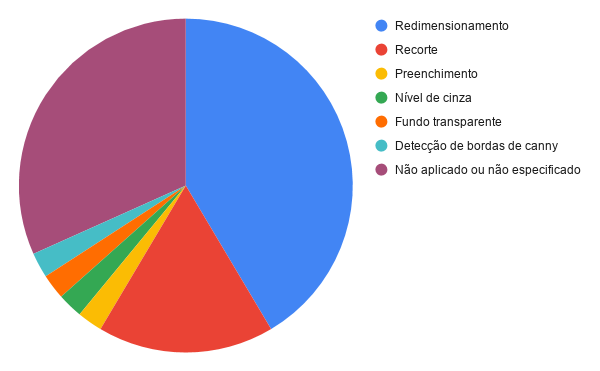
\includegraphics[scale=.60]{imagens/revisao_sistematica/grafico_preprocessamento_vs_uso.png}
    \label{fig:grafico_preprocessamento_vs_uso}
    \source{Danilo Assunção, 2021}
\end{figure}

O desempenho da tarefa de classificação é melhorado ao aplicar as técnicas de pré-processamento de imagem para extrair automaticamente o resultado da imagem introduzida antes de ser inserida nos modelos de aprendizagem profunda \cite{thenmozhi2019crop}. A técnica de Redimensionamento (\textit{resize}) vem liderando com 41,46\% de uso com relação as outras estratégias abordadas, e isso se deve aos diversos fatores que auxiliam no aumento de performance das redes neurais convolucionais, como a quantidade reduzida de parâmetros a serem introduzidos na rede. Em segundo com 17,07\%, o Recorte (\textit{cropping}) que pode vir a ser utilizado para destacar a região de interesse da imagem e reduzindo também o tamanho da imagem \cite{thenmozhi2019crop}. Preenchimento (\textit{padding}), Nível de cinza (\textit{gray scale}), Fundo transparente (\textit{transparent background}) e Detecção de bordas de canny (\textit{canny edge detection}) foram algumas das abordagens utilizadas, e ocupam apenas 2,44\% de uso com relação aos outros métodos. Ocupando os 31,71\% restantes, foram artigos que não aplicaram ou não especificaram diretamente o uso de técnicas de pré-processamento de imagens, isto pode ser ocasionado pelo fato do conjunto de dados utilizado já estar previamente pré-processado em sua disponibilização, ou de não haver necessidade direta de uma preparação antes de introduzi-las à rede.

\subsection{Técnica de aprendizado por transferência}
Aprendizado por transferência (\textit{Transfer learning}) é uma técnica que permite a utilização de uma rede pré-treinada, reduzindo a carga computacional e beneficiando-se do poder de uma rede neural convolucional mais sofisticada \cite{valan2019automated}. 

Dois métodos foram comumente utilizados como técnicas de aprendizado por transferência, sendo elas, o ajuste fino e a transferência de características. O ajuste fino (\textit{fine-tuning}) modifica os parâmetros de uma Rede Neural Convolucional pré-treinada para o treinamento de uma nova tarefa, onde a camada de saída é estendida com pesos inicializados aleatoriamente para a nova tarefa, e uma pequena taxa de aprendizagem é usada para ajustar os parâmetros de seus valores originais para minimizar a perda no novo modelo \cite{li2017learning}. A transferência de características (\textit{feature transfer}) faz uso de uma rede neural convolucional pré-treinada para calcular recursos para uma imagem \cite{li2017learning}. A extração de recursos não modifica a rede original e permite que novas tarefas se beneficiem de recursos complexos aprendidos em tarefas anteriores \cite{li2017learning}.

Na Figura \ref{fig:grafico_transfer-learning_vs_uso} será apresentado os dados coletados por meio dos artigos analisados que utilizam de técnicas de aprendizado por transferência, na resolução de cenários que abordam o uso de Redes Neurais Convolucionais.

\begin{figure}[H]
    \centering
    \caption{Técnicas de Aprendizado por transferência}
    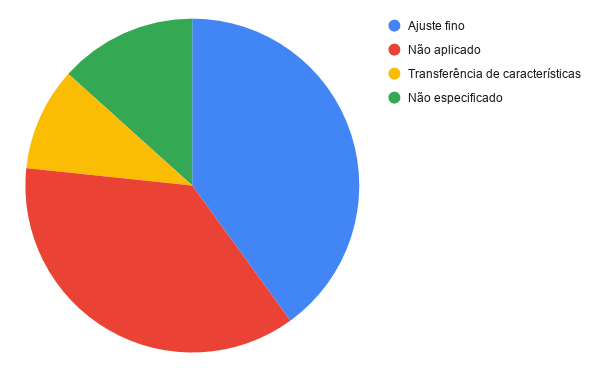
\includegraphics[scale=.60]{imagens/revisao_sistematica/grafico_transfer-learning_vs_uso.png}
    \label{fig:grafico_transfer-learning_vs_uso}
    \source{Danilo Assunção, 2021}
\end{figure}

O ajuste fino foi o método mais utilizado com 40,00\% (12) de uso em relação a todas as outras técnicas encontradas nos artigos analisados. Podendo ser devido ao ajuste fino funcionar bem quando o modelo especializado é semelhante à nova tarefa proposta \cite{valan2019automated}, e este mecanismo foi utilizado para diversas tarefas com cenários semelhantes de reconhecimento de padrões. Em segundo, é tido em todos os artigos que não aplicaram nenhuma técnica de Aprendizado por transferência ocupando 36,67\% (11), devendo-se ao fato de que nem todo cenário pode vir a necessitar do uso de técnica de reaproveitamento deste tipo, e também, este mecanismo é suscetível a sobreajuste na tarefa especializada quando os conjuntos de dados são pequenos, pois pode associar incorretamente uma categoria rara a um recurso irrelevante, como um tipo especial de fundo, que por acaso está presente nas poucas imagens dessa categoria e no conjunto de treinamento \cite{valan2019automated}. O método de transferência de características teve um uso de 10,00\% (3) com relação às outras técnicas abordadas. O restante mapeado, com 13,33\% (4) não especificou diretamente o tipo de mecanismo de Aprendizado por transferência utilizado.

\subsection{Técnicas de aumento de dados}
Métodos de Aumento de dados (\textit{Data augmentation}) permite aumentar artificialmente o tamanho do conjunto de treinamento. O aumento do conjunto de treinamento é feito ao aplicar várias distorções às imagens originais, como zoom, virando-as horizontalmente ou verticalmente, girando-as, deslocando-as e dentre outros \cite{gomez2019coral}. Na Figura \ref{fig:grafico_aumento-dados_vs_uso} é demonstrado graficamente as técnicas utilizadas para o Aumento de dados nos artigos abordados.

\begin{figure}[H]
    \centering
    \caption{Técnicas de Aumento de dados}
    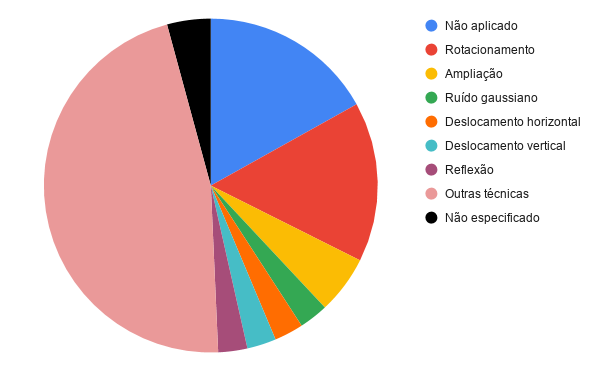
\includegraphics[scale=.60]{imagens/revisao_sistematica/grafico_aumento-dados_vs_uso.png}
    \label{fig:grafico_aumento-dados_vs_uso}
    \source{Danilo Assunção, 2021}
\end{figure}

Em maioria, os artigos não aplicaram técnicas de Aumento de dados, com uma representação de 16,90\% (12) de todos os exemplares analisados, isto pode ser ocasionado pelo fato dos conjuntos de dados utilizados pelos autores já forem grandes o suficiente ou devido ao uso de outras técnicas para supressão de sobreajuste. Em seguida, é possível observar que as técnicas de Aumento de dados utilizando Rotacionamento (\textit{Rotation}) são bem prioritárias quando este mecanismo é aplicado, com um total de uso de 15,49\% (11) com relação aos outros meios. Ampliação (\textit{Zooming}), sendo a terceira metodologia mais aplicada com 5,63\% (4). Ruído gaussiano (\textit{Gaussian noise}), Deslocamento horizontal (\textit{Width shifting}), Deslocamento vertical (\textit{Height shifting}) e Reflexão (\textit{Reflection}) representando 2,82\% (2) nos demais cenários. As Outras técnicas agrupadas são métodos que foram utilizados somente uma única vez e o conjunto não especificado são aos artigos que não esclareceram de maneira explicita o tipo de técnica de Aumento de dados utilizada.

\subsection{Modelo de arquitetura da CNN}
É possível identificar na literatura uma grande quantidade de arquiteturas de Redes Neurais Convolucionais sendo utilizadas em diversas soluções de problemas que envolvem a classificação morfológica de espécies, por meio de suas imagens digitais. Na Figura \ref{fig:grafico_arquitetura_vs_uso} é possível observar graficamente estes dados.

\begin{figure}[H]
    \centering
    \caption{Arquitetura de Redes Neurais Convolucionais}
    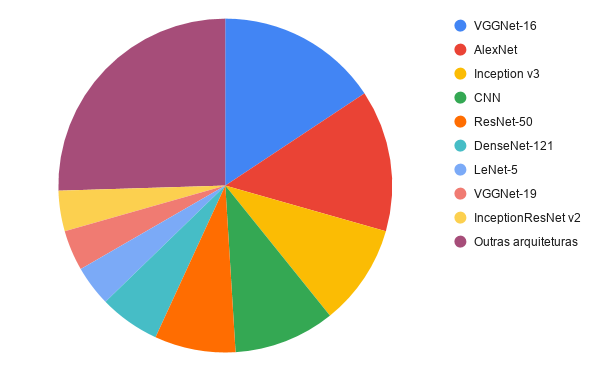
\includegraphics[scale=.60]{imagens/revisao_sistematica/grafico_arquitetura_vs_uso.png}
    \label{fig:grafico_arquitetura_vs_uso}
    \source{Danilo Assunção, 2021}
\end{figure}

A VGGNet-16 obteve uma utilização de 14,29\% (8), encontrando-se em primeiro com relação as outras arquiteturas destacadas. Em comparação a AlexNet posicionada em segundo com 12,50\% (7), as arquiteturas de VGGNet aumentam a profundidade da rede e reduz o tamanho do \textit{kernel} de convolução, podendo assim reduzir os parâmetros a serem computados, além disso, o desempenho de generalização de arquiteturas VGGNet costumam ter bons resultados \cite{li2020using}. Os modelos de Inception v3 e CNN, onde a categoria CNN representa os modelos implementados pelos autores em seus artigos ocupam 7,81\% (5). ResNet-50 com 6,25\% (4) e DenseNet-121 com 4,69\% (3). LeNet-5, VGGNet-19 e InceptionResNet v2 que ocupam 3,13\% (2) em aplicabilidade. Já as ``Outras arquiteturas'' que compõe 20,31\% do restante das arquiteturas utilizadas, possuem uma única utilização em seus respectivos artigos.

Para uma diferente perspectiva de visualização de usabilidade das arquiteturas de Redes Neurais Convolucionais extraídas nos projetos em questão, foi feito um agrupamento por tipo de arquitetura para a identificação dos exemplares mais utilizados, como é demonstrado na Figura \ref{fig:grafico_arquitetura_agrupada_vs_uso}.

\begin{figure}[H]
    \centering
    \caption{Tipos agrupados de arquiteturas de Redes Neurais Convolucionais}
    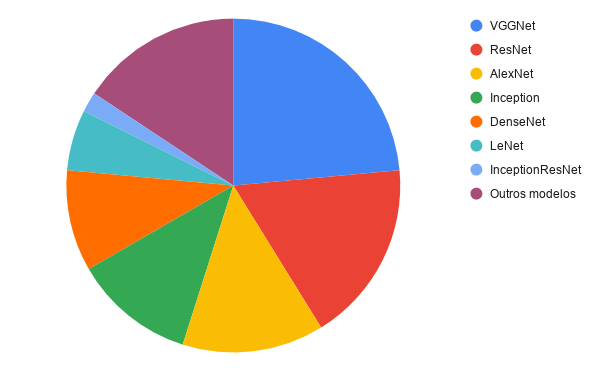
\includegraphics[scale=.60]{imagens/revisao_sistematica/grafico_arquitetura_agrupada_vs_uso.png}
    \label{fig:grafico_arquitetura_agrupada_vs_uso}
    \source{Danilo Assunção, 2021}
\end{figure}

Nota-se que modelos de VGGNet com uso de 23,53\% (12) ainda dominam em termos de arquiteturas aplicadas na resolução de problemas envolvendo a identificação de espécies. Arquiteturas do tipo ResNet ocupam o segundo lugar com 17,65\% (9), isso devido ao seu comportamento de aumentar a profundidade da rede, sendo assim, as ResNets oferecem melhores recursos de aproximação de função (convergência ao resultado) à medida em que ganham mais parâmetros, contribuindo com sucesso na resolução de problemas como os de dissipação de gradiente, onde alguns modelos mais tradicionais acabam não conseguindo soluciona-lo, tendo resultados inferiores ao desejado \cite{sun2017deep}. Tendo a AlexNet em terceiro com 13,73\% (7), sendo este tipo de arquitetura um modelo pré-treinado de rede neural convolucional que permite a aplicação de Aprendizado por Transferência para que atinja melhores resultados \cite{hongclassification}. Modelos de Inception 11,76\% (6), DenseNet 9,80\% (5). LeNet 5,88\% (5) e InceptionResNet 1,96\% (1) possuem a menor quantidade de uso para os cenários avaliados. Por último, os ``Outros modelos'' que são arquiteturas de CNN desenvolvidas pelos autores dos artigos com especificidade para solucionar seus respectivos problemas abordados.

\subsection{Modelo do classificador}
Os métodos de classificação são aplicados nas últimas camadas das Redes Neurais Convolucionais, utilizando as características extraídas como entrada para o processo de classificação dos dados e predição do resultado. Na Figura \ref{fig:grafico_classificador_vs_uso} é demonstrado os exemplares aplicados nos artigos selecionados.

\begin{figure}[H]
    \centering
    \caption{Método de classificação utilizado}
    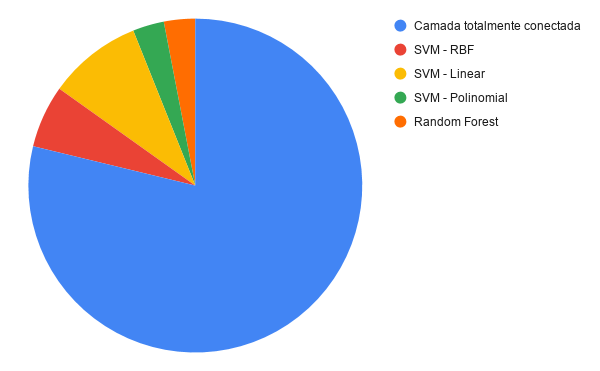
\includegraphics[scale=.60]{imagens/revisao_sistematica/grafico_classificador_vs_uso.png}
    \label{fig:grafico_classificador_vs_uso}
    \source{Danilo Assunção, 2021}
\end{figure}


A partir do processo de convolução da Rede Neural Convolucional, é seguido o agrupamento e divisão das imagens em recursos. Em sequência desse processo, tais recursos são utilizados para alimentar a estrutura de rede neural totalmente conectada, pode direcionar a decisão de classificação final \cite{rauf2019visual}. 

Decorrendo em 78,79\% (26) de utilização apresentada nos artigos e representada como ``Camada totalmente conectada''. Nos demais cenários onde a rede neural convolucional é utilizada somente para extração de características, é visto a aplicação conjunta com algoritmos de SVM (Máquina de vetores de suporte) com \textit{kernel} Linear 9,09\% (3), RBF (Função de Base Radial) 6,06\% (2) e Polinomial 3,03\% (1). Por fim, houve apenas uma implementação do algoritmo \textit{Random Forest} ocupando 3,03\% (1).

\section{Conclusão}
Após o término da revisão sistemática é perceptível que o uso de técnicas de aprendizado profundo, como redes neurais convolucionais, vem sendo empregadas em diversos cenários onde há a necessidade de otimização no processo de extração de características das imagens, para assim, solucionar problemas que envolvem reconhecimento de espécies. Um dos atributos mais importantes é a sua capacidade de aprender as características de mais alto nível de uma imagem, e fornecer prontamente uma quantidade de informações relevantes que permitam que os algoritmos de classificação possam identificar com mais eficácia o objeto visualizado. Entretanto, é importante ressaltar que o uso deste mecanismo exige uma quantidade muito grande de dados, justamente para que seu resultado venha a convergir para um modelo que tenha a capacidade de efetivar tal atividade, e para isto foi observado na literatura o uso de técnicas como transferência de aprendizado e aumento de dados que permitem a utilização de redes neurais convolucionais, mesmo com um conjunto pequeno de dados disponíveis e demonstrando também que o uso de pré-processamento ainda pode vir a ser extremamente útil em cenários diversos envolvendo processamento de imagens digitais.

\chapter{Materiais e métodos}
Visando a atingir o objetivo desta pesquisa, serão conduzidos experimentos com base em um conjunto de dados de treinamento e de validação, unindo técnicas de aprendizado por transferência ou aumento de dados aplicados a uma rede neural convolucional, contendo uma estrutura para a extração de características e classificação supervisionada das imagens das asas de maneira automática.
No conjunto de treinamento e validação, serão utilizadas as imagens de asas de abelhas obtidas em um ângulo que mostre a face da asa, de tal maneira a expor claramente suas nervuras, como pode ser visto na Figura \ref{fig:02_mel_trigona_spinipes}. As imagens contidas nos conjuntos de dados já foram previamente rotuladas com a espécie da abelha por um especialista da área.

\begin{figure}[H]
    \centering
    \caption{Imagem das nervuras destacadas de uma asa de abelha}
    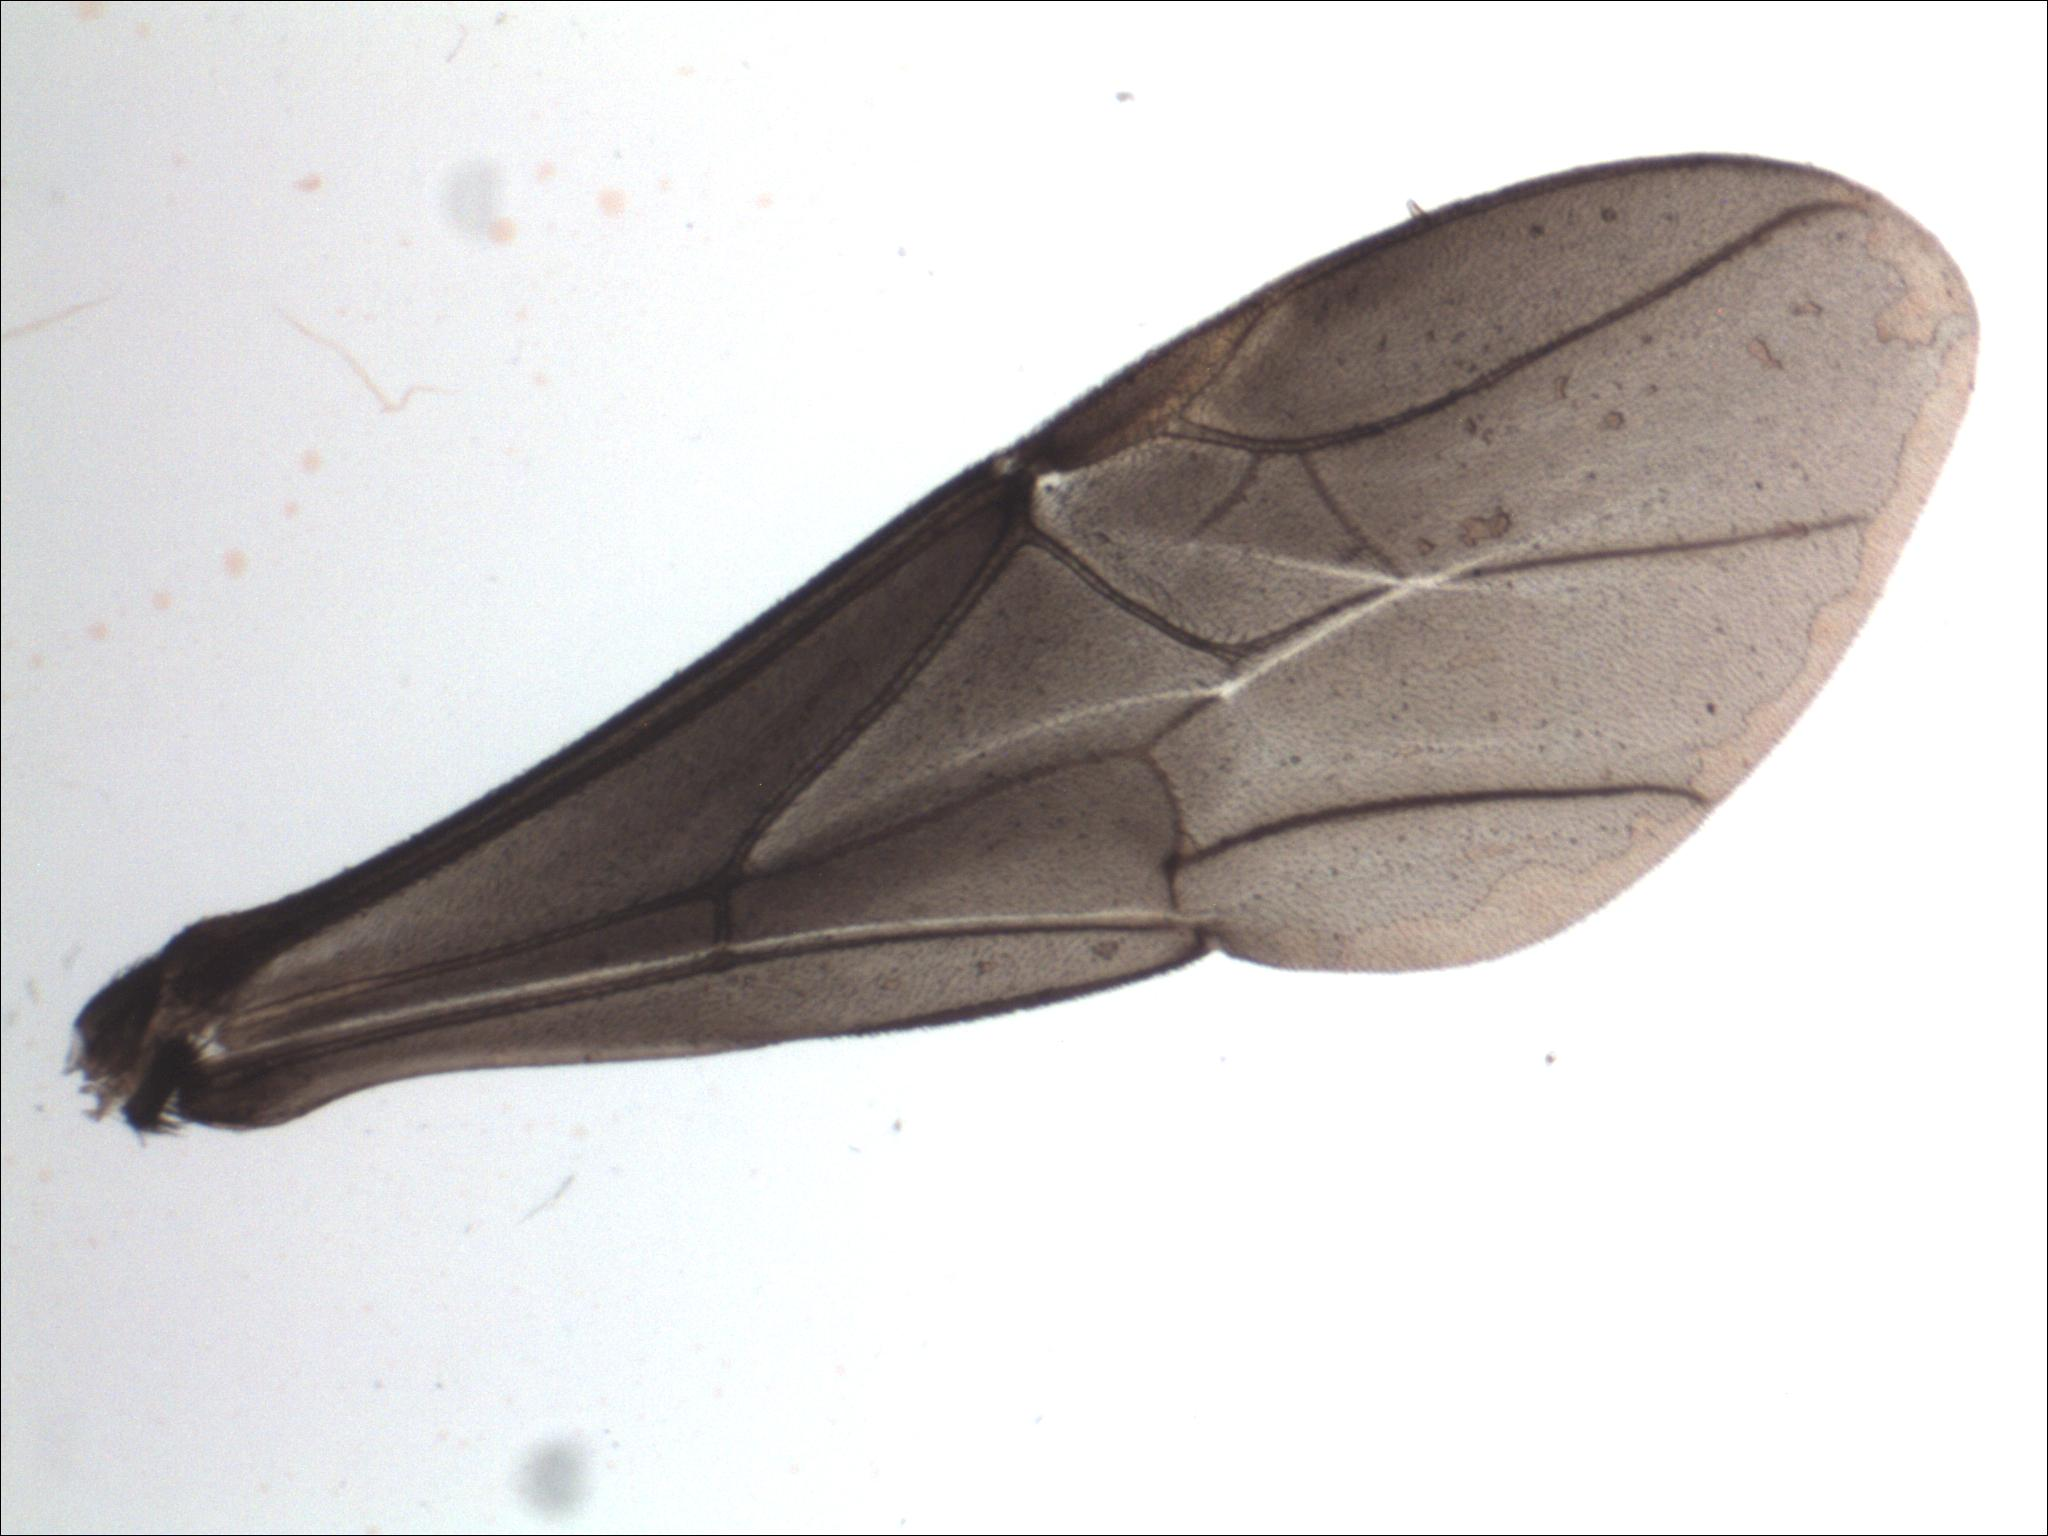
\includegraphics[width=.45\textwidth]{imagens/materiais_metodos/02_mel_trigona_spinipes.jpg}\hfill
    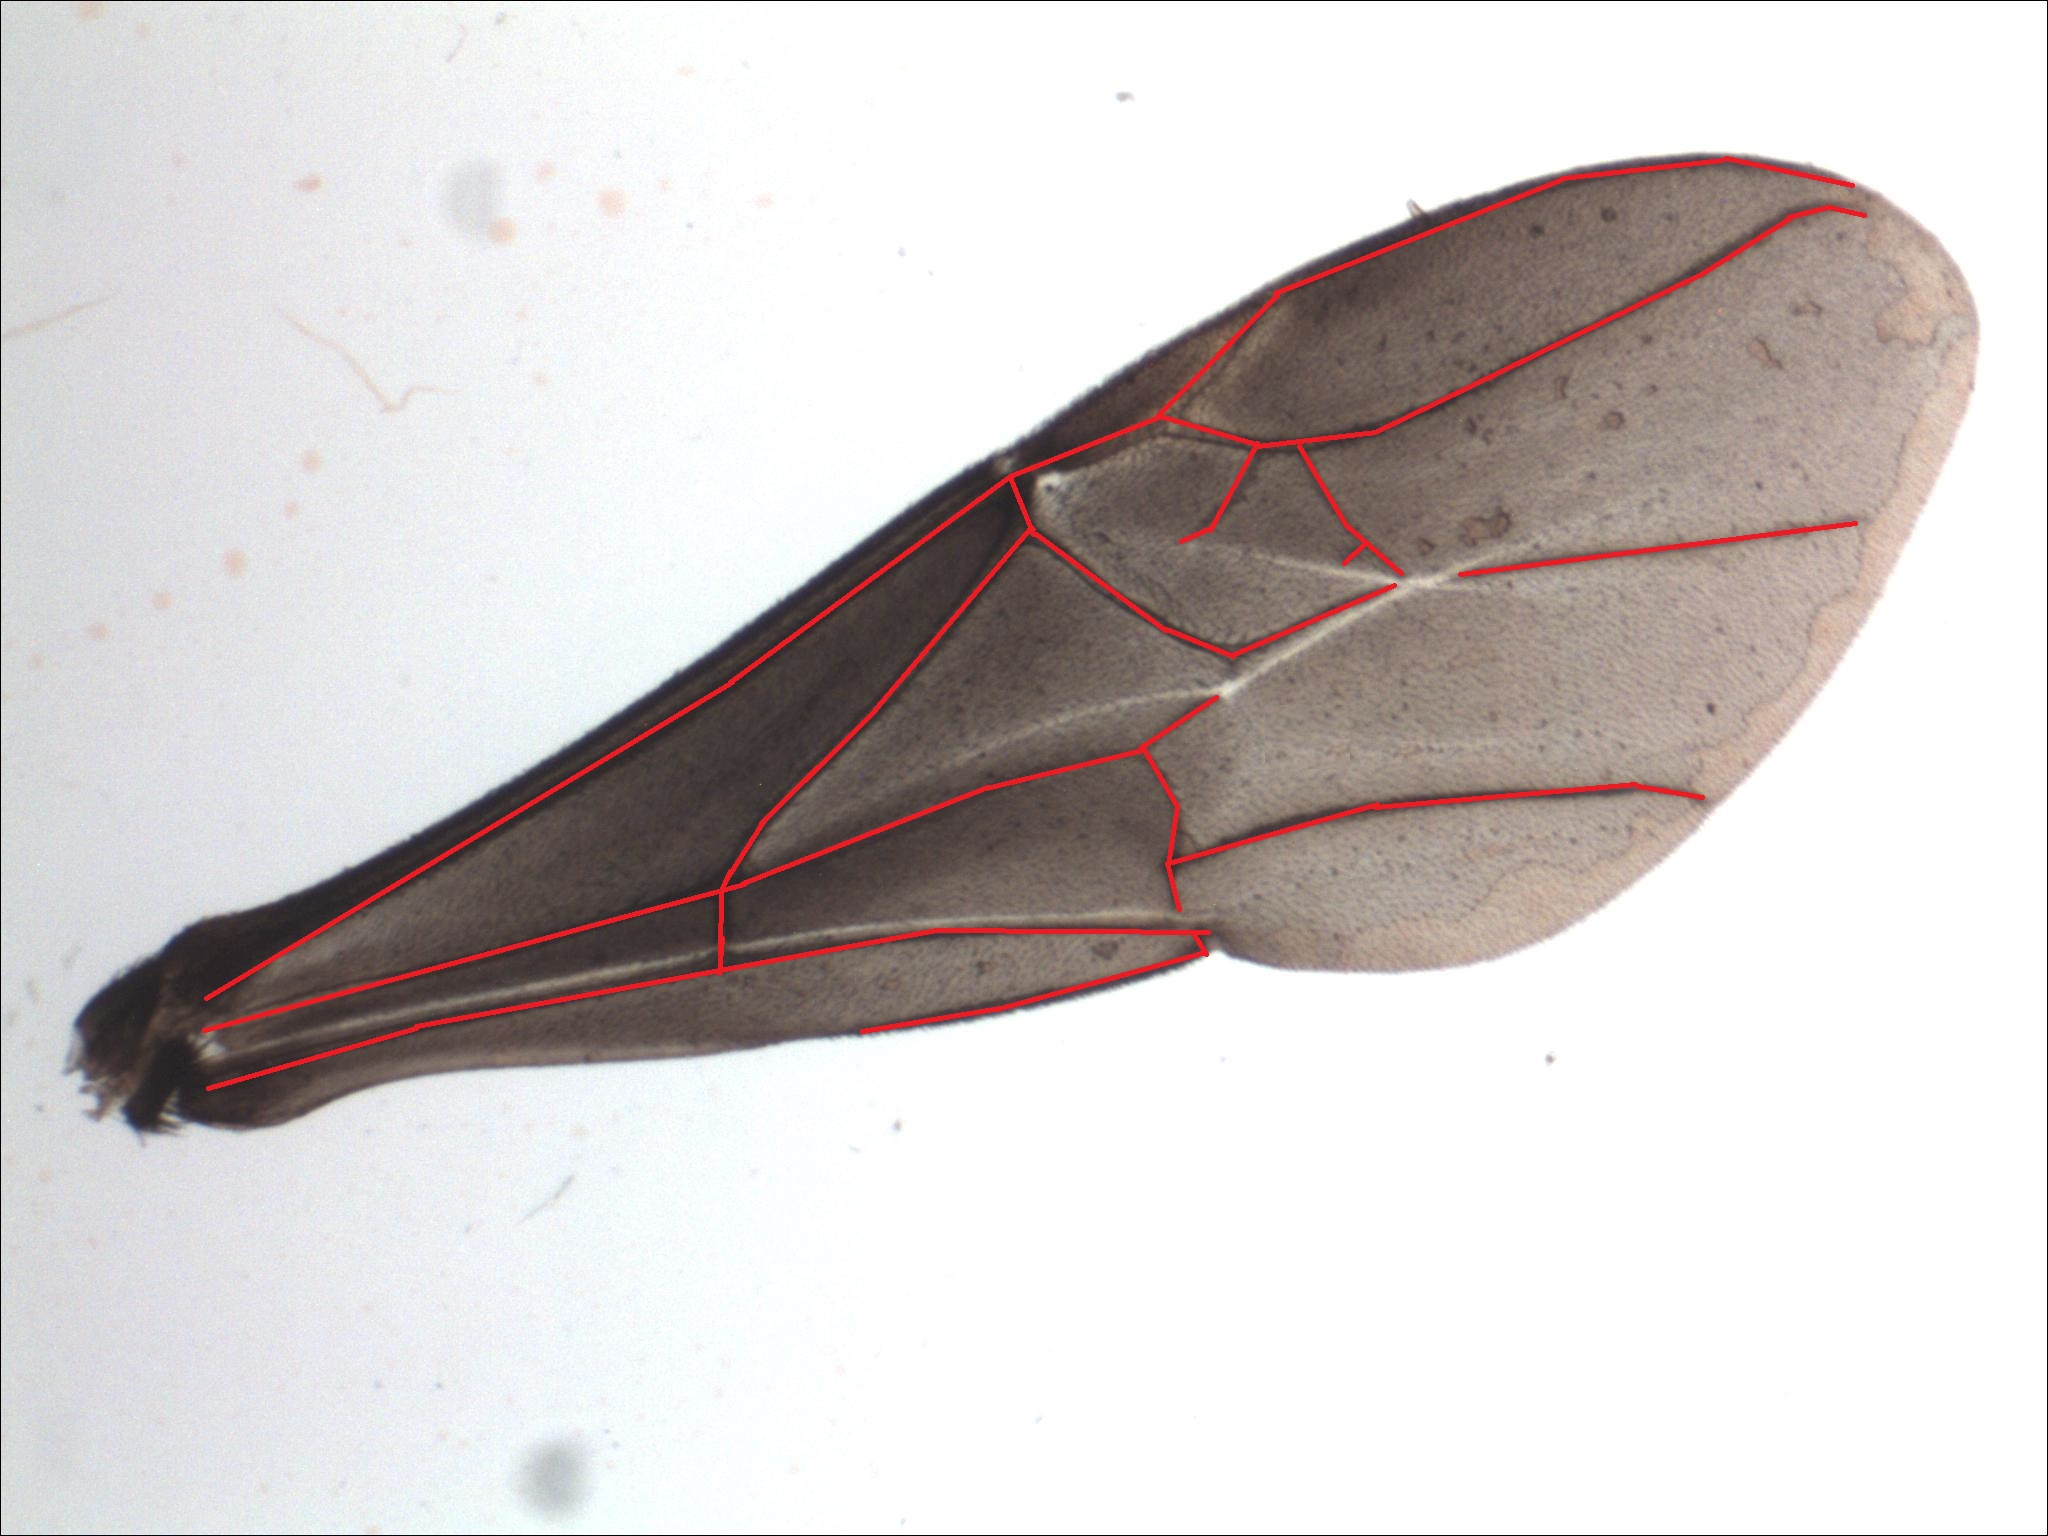
\includegraphics[width=.45\textwidth]{imagens/materiais_metodos/02_mel_trigona_spinipes_mapped.jpg}
    \label{fig:02_mel_trigona_spinipes}
    \source{Danilo Assunção, 2021}
\end{figure}

Para levantar o estado da arte das técnicas de aprendizado por transferência, aumento de dados e CNN, foi elaborada uma revisão sistemática utilizando os conceitos aplicados em \citeonline{liu2020classification}.

Após o levantamento do estado da arte como base, pretende-se construir uma CNN como ferramenta de classificação, empregando as melhores técnicas obtidas e, em caso pertinente, uma combinação do uso de técnicas de aprendizado por transferência ou aumento de dados, devem ser introduzidas, a fim de melhorar o estado da arte do método aplicado.

\section{Ferramenta de classificação}
O processo definido para a elaboração da ferramenta de classificação, utilizando imagens das asas de abelhas, está dividido em quatro partes principais:

\begin{enumerate}
  \item Pré-processamento;
  \item Carregamento;
  \item Extração das características;
  \item Classificação.
\end{enumerate}

No pré-processamento, serão feitas as aplicações necessárias de processamento de imagem, nas imagens do conjunto de dados, para tratamentos gerais como, a dimensão da imagem, recorte e a possível aplicação de técnicas de aumento de dados, para a geração de um conjunto maior de dados. No passo de carregamento, a imagem pré-processada será transformada em uma representação computacional, a qual a CNN consiga computar e aceitar como valor de entrada. No processo de extração de características, os dados passarão pela arquitetura da CNN, onde será feito todo o processo convolucional junto ao redimensionamento dos dados dessa imagem, até a extração das melhores características destas imagens. Por fim, o processo de classificação será responsável pelo mecanismo de descriminação das espécies, por meio das características adquiridas no passo anterior.

A etapa de classificação contará com dois passos essenciais, o treinamento e classificação. No treinamento será utilizado um conjunto misto de dados, intitulados como conjunto de treinamento e validação para treinamento da camada de classificação da CNN, e um conjunto de teste deverá ser aplicado em cima do resultado obtido pela rede, para a visualização e confirmação do valores deferidos na saída deste procedimento.

\section{Avaliação}
A avaliação é executada ao comparar os resultados produzidos automaticamente pela CNN, observando a aplicação de métricas de aprendizado de máquina supervisionado (revocação, precisão, acurácia), para assim mensurar os resultados obtidos no processo de discriminação das classes.

%------------------------------------------------------------------------
% CAPITULO - PROPOSTA DE PESQUISA
%------------------------------------------------------------------------
\chapter{Proposta de pesquisa}
Na literatura foi possível observar que, o processo de extração manual de características das imagens é algo fundamental para um melhor desempenho na classificação, mas é tida como uma tarefa especializada e trabalhosa. Muitos desses recursos de mais alto nível acabam por não poder ser extraídos manualmente ao utilizar apenas de métodos de segmentação. Sendo assim, um procedimento que permita determinar automaticamente os recursos adequados para um deliberado problema, que envolva a identificação por meio de imagens vem sendo muito requisitado  \cite{waldchen2018machine}. No campo da ecologia, uma das tarefas é a identificação de espécias de abelhas a partir de imagens de suas asas \cite{liu2020classification}, visto que a combinação de técnicas que envolvem o mecanismo de aprendizado profundo é raramente explorado \cite{liu2020classification}. Entretanto, pesquisadores têm demonstrado, nos últimos anos, um aumento no interesse pela área de aprendizado de máquina, na qual a construção de sistemas de classificação de espécies mais eficientes, que utilizam técnicas de aprendizagem de máquina, acaba por ser de grande interesse e aplicabilidade no ramo científico \cite{liu2020classification}. Para a aplicação de uma CNN na resolução de problemas envolvendo imagens e reconhecimento de espécies, é necessário uma quantidade maior de dados para que a rede consiga convergir para um bom quadro de hipóteses, permitindo alcançar melhores resultados no processo de reconhecimento. Portanto, dois problemas ocorrem no treinamento destes modelos em conjunto de dados ecológicos, sendo eles o conjunto de dados de imagens limitado e os números de amostras desequilibrados entre as diferentes classes, dessa maneira, as precisões de teste para os modelos de CNN existentes no conjunto de dados ecológicos podem ser baixas \cite{liu2020classification}. Visando a resolver os problemas mencionados, neste trabalho será utilizada uma CNN para, assim, realizar a extração automática das características contidas na morfologia das asas das abelhas presentes em imagens digitais. A partir destas caraterísticas, identificar as respectivas espécies, em conjunto à técnicas de aumento de dados na série de imagens disponibilizadas, com o intuito de ampliar em diversas vezes o seu tamanho, visando também a elevar a eficiência da velocidade de convergência da rede a partir de técnicas de aprendizado por transferência. Almeja-se, assim, um melhor desempenho nos resultados desejados para o processo de classificação das espécies de abelhas.

\section{Plano de trabalho e cronograma}
A seguir são apresentados um cronograma representado pela Tabela \ref{tab:cronograma} e todas as atividades que englobam este projeto de pesquisa:

\begin{enumerate}
  \item Revisão bibliográfica: uma revisão sistemática da literatura foi realizada a fim de identificar o estado da arte do uso de CNN, com técnicas que proveem um mecanismo que permita o uso deste tipo de rede em diversos cenários para a identificação de espécies;
  \item Teste de proficiência em inglês: realização da prova de proficiência em inglês solicitada pelo programa;
  \item Qualificação: realização do exame de qualificação;
  \item Preparação dos dados: levantamento de todo o conjunto de dados das abelhas disponível contendo imagens de suas asas e aplicação de possíveis técnicas de aumento de dados para ampliação deste conteúdo.
  \item Preparação do modelo de CNN: definição e desenvolvimento de um algoritmo de CNN para o modelo;
  \item Extração de características: aplicação da CNN desenvolvida para extração de características, podendo ser utilizadas técnicas de aprendizado por transferência;
  \item Classificação: compilado do resultado obtido no passo de extração em um algoritmo de classificação supervisionado estabelecido na CNN;
  \item Avaliação: testes utilizando os algoritmos de classificação propostos para identificação das imagens;
  \item Escrita da dissertação;
  \item Defesa.
\end{enumerate}


%----------------------------------------------------
% TABELA - CRONOGRAMA
%----------------------------------------------------
\begin{table}[H]
\centering
\caption{Cronograma}
\label{tab:cronograma}
\resizebox{\textwidth}{!}{%
\begin{tabular}{|l|l|l|l|l|l|l|l|l|l|l|l|l|l|l|l|l|l|l|l|l|l|l|}
\hline
\multicolumn{2}{|l|}{Atividade}     & \multicolumn{5}{l|}{2020} & \multicolumn{12}{l|}{2021}                       & \multicolumn{4}{l|}{2022} \\ \hline
\#   & Descrição                       & 8  & 9  & 10  & 11  & 12  & 1 & 2 & 3 & 4 & 5 & 6 & 7 & 8 & 9 & 10 & 11 & 12 & 1    & 2    & 3    & 4    \\ \hline
1  & Revisão bibliográfica           & x  & x  & x   & x   & x   & x & x & x & x &   &   &   &   &   &    &    &    &      &      &      &      \\ \hline
2  & Teste de proficiência em inglês &    &    &     &     &     &   &   &   &   & x &   &   &   &   &    &    &    &      &      &      &      \\ \hline
3  & Qualificação                    &    &    &     &     &     &   &   &   & x &   &   &   &   &   &    &    &    &      &      &      &      \\ \hline
4  & Preparação dos dados            &    &    &     &     &     &   &   &   &   & x & x & x & x & x &    &    &    &      &      &      &      \\ \hline
5  & Preparação do modelo CNN        &    &    &     &     &     &   &   &   &   &   &   & x & x & x &    &    &    &      &      &      &      \\ \hline
6  & Extração de características     &    &    &     &     &     &   &   &   &   &   &   &   &   & x & x  & x  &    &      &      &      &      \\ \hline
7  & Classificação                   &    &    &     &     &     &   &   &   &   &   &   &   &   & x & x  & x  &    &      &      &      &      \\ \hline
8  & Avaliação                       &    &    &     &     &     &   &   &   &   &   &   &   &   &   &    & x  & x  &      &      &      &      \\ \hline
9  & Escrita da dissertação            &    &    &     &     &     &   &   &   &   &   &   & x & x & x & x  & x  & x  & x    & x    & x    &      \\ \hline
10 & Defesa                          &    &    &     &     &     &   &   &   &   &   &   &   &   &   &    &    &    &      &      &      & x    \\ \hline
\end{tabular}%
}
\source{Danilo Assunção, 2021}
\end{table}

\chapter{Considerações finais}
Este trabalho propõe a utilização de visão computacional para a construção de um modelo de CNN, o qual realize o reconhecimento de espécies de abelhas a partir da morfologia de suas asas presentes em imagens digitais. Pretende-se utilizar conjunto a este mecanismo, técnicas de aumento de dados ou aprendizado por transferência. Inicialmente, foi realizada uma revisão sistemática da literatura, que identificou as técnicas de aumento de dados e aprendizado por transferência utilizando CNN para tarefas de reconhecimento de espécies. Esta revisou permitiu o entendimento das diversas possibilidades disponíveis para a aplicação de técnicas de aprendizado profundo, mesmo quando se tem poucos dados disponíveis, o que permite uma maior autonomia e flexibilidade no colhimento das características das imagens, junto a uma automatização como um todo no processo de reconhecimento. Com este método, espera-se obter bons resultados na classificação das espécies de abelhas, utilizando um modelo de CNN como automatizador de todo o processo de extração e classificação deste domínio.

% ----------------------------------------------------------
% ELEMENTOS PÓS-TEXTUAIS
% ----------------------------------------------------------
\postextual
% ----------------------------------------------------------

% ----------------------------------------------------------
% Referências bibliográficas
% ----------------------------------------------------------
\bibliography{referencias}

% ----------------------------------------------------------
% Glossário
% ----------------------------------------------------------
%
% Consulte o manual da classe abntex2 para orientações sobre o glossário.
%
%\glossary

% ----------------------------------------------------------
% Apêndices
% ----------------------------------------------------------

% ---
% Inicia os apêndices
% ---
% \begin{apendicesenv}

% Imprime uma página indicando o início dos apêndices
%\partapendices

%-------------------------------------------------------------------------
% Comentário adicional do PPgSI - Informações sobre ``apêndice''
%
% Para todos os captions/(títulos) (de seções, subseções, tabelas, 
% ilustrações, etc.):
%     - em maiúscula apenas a primeira letra da sentença (do título), 
%       exceto nomes próprios, geográficos, institucionais ou Programas ou
%       Projetos ou siglas, os quais podem ter letras em maiúscula também.
%
% Todas  as tabelas, ilustrações (figuras, quadros, gráficos etc. ), 
% anexos, apêndices devem obrigatoriamente ser citados no texto.
%      - a citação deve vir sempre antes da primeira vez em que a tabela, 
%        ilustração etc., aparecer pela primeira vez.
%
%-------------------------------------------------------------------------

% \end{apendicesenv}
% ---


% ----------------------------------------------------------
% Anexos
% ----------------------------------------------------------

% ---
% Inicia os anexos
% ---
% \begin{anexosenv}

% Imprime uma página indicando o início dos anexos
%\partanexos


%-------------------------------------------------------------------------
% Comentário adicional do PPgSI - Informações sobre ``anexo''
%
% Para todos os captions/(títulos) (de seções, subseções, tabelas, 
% ilustrações, etc.):
%     - em maiúscula apenas a primeira letra da sentença (do título), 
%       exceto nomes próprios, geográficos, institucionais ou Programas ou
%       Projetos ou siglas, os quais podem ter letras em maiúscula também.
%
% Todas  as tabelas, ilustrações (figuras, quadros, gráficos etc. ), 
% anexos, apêndices devem obrigatoriamente ser citados no texto.
%      - a citação deve vir sempre antes da primeira vez em que a tabela, 
%        ilustração etc., aparecer pela primeira vez.
%
%-------------------------------------------------------------------------

% \end{anexosenv}

\end{document}